\documentclass[11pt,oneside,openany]{book}

% ---------------------------------------------------------------------------
% PAGE GEOMETRY & TYPOGRAPHY
% ---------------------------------------------------------------------------
\usepackage[a4paper,top=2.2cm,bottom=2.3cm,left=2.0cm,right=2.0cm,headheight=16pt]{geometry}
\usepackage[T1]{fontenc}
\usepackage[utf8]{inputenc}
\usepackage{lmodern}
\usepackage{microtype}
\usepackage{emptypage}

% ---------------------------------------------------------------------------
% MATHEMATICS PACKAGES
% ---------------------------------------------------------------------------
\usepackage{amsmath,amssymb,amsfonts,bm}
\usepackage{mathtools}
\usepackage{mathrsfs}

% ---------------------------------------------------------------------------
% GRAPHICS, TIKZ & TABLES
% ---------------------------------------------------------------------------
\usepackage{graphicx}
\graphicspath{{figures/}{images/}}
\usepackage{xcolor}
\usepackage{tikz}
\usetikzlibrary{arrows.meta,positioning,calc,patterns,shapes}
\usepackage{booktabs}
\usepackage{array}
\usepackage{longtable}
\usepackage{enumitem}
\usepackage{caption}
\captionsetup{font=small,labelfont={bf,color=navyblue},width=0.92\textwidth}

% ---------------------------------------------------------------------------
% COLOR PALETTE (Authoritative Academic Palette)
% ---------------------------------------------------------------------------
\definecolor{navyblue}{HTML}{0F2A4A}
\definecolor{accentcrimson}{HTML}{8C1D40}
\definecolor{forestgreen}{HTML}{134E3F}
\definecolor{ambergold}{HTML}{B45309}
\definecolor{slateink}{HTML}{1F2937}
\definecolor{lightgraybg}{HTML}{F8FAFC}
\definecolor{borderblue}{HTML}{1E40AF}
\definecolor{softgreen}{HTML}{F0FDF4}
\definecolor{softred}{HTML}{FEF2F2}
\definecolor{softblue}{HTML}{F0F7FF}
\definecolor{softamber}{HTML}{FFFBEB}
\definecolor{gridblue}{HTML}{CBD5E1}

% ---------------------------------------------------------------------------
% CALLOUT BOXES & THEOREMS (tcolorbox)
% ---------------------------------------------------------------------------
\usepackage{tcolorbox}
\tcbuselibrary{skins,breakable}

% Definition Box
\newtcolorbox{definitionbox}[1]{
  enhanced, breakable, colback=softblue, colframe=navyblue,
  boxrule=0.6pt, leftrule=4pt, arc=2pt, left=10pt, right=10pt, top=7pt, bottom=7pt,
  fonttitle=\sffamily\bfseries\small,
  title={\textsc{Definition} \enspace\textperiodcentered\enspace #1},
  coltitle=white, colbacktitle=navyblue
}

% Theorem Box
\newtcolorbox{theorembox}[1]{
  enhanced, breakable, colback=softred, colframe=accentcrimson,
  boxrule=0.6pt, leftrule=4pt, arc=2pt, left=10pt, right=10pt, top=7pt, bottom=7pt,
  fonttitle=\sffamily\bfseries\small,
  title={\textsc{Theorem} \enspace\textperiodcentered\enspace #1},
  coltitle=white, colbacktitle=accentcrimson
}

% Proposition / Lemma Box
\newtcolorbox{propbox}[1]{
  enhanced, breakable, colback=softgreen, colframe=forestgreen,
  boxrule=0.6pt, leftrule=4pt, arc=2pt, left=10pt, right=10pt, top=7pt, bottom=7pt,
  fonttitle=\sffamily\bfseries\small,
  title={\textsc{Proposition / Lemma} \enspace\textperiodcentered\enspace #1},
  coltitle=white, colbacktitle=forestgreen
}

% Historical Context Box
\newtcolorbox{historicalbox}[1]{
  enhanced, breakable, colback=softamber, colframe=ambergold,
  boxrule=0.6pt, leftrule=4pt, arc=2pt, left=10pt, right=10pt, top=7pt, bottom=7pt,
  fonttitle=\sffamily\bfseries\small,
  title={\textsc{Historical Milestone} \enspace\textperiodcentered\enspace #1},
  coltitle=white, colbacktitle=ambergold
}

% Worked Example Box (Auto counter)
\newtcolorbox[auto counter, number within=chapter]{workedexample}[1]{
  enhanced, breakable, colback=lightgraybg, colframe=borderblue,
  boxrule=0.6pt, leftrule=4pt, arc=2pt, left=10pt, right=10pt, top=7pt, bottom=7pt,
  fonttitle=\sffamily\bfseries\small,
  title={\textsc{Worked Example \thetcbcounter} \enspace\textperiodcentered\enspace #1},
  coltitle=white, colbacktitle=borderblue
}

% ---------------------------------------------------------------------------
% HEADERS, FOOTERS & TITLES
% ---------------------------------------------------------------------------
\usepackage{titlesec}
\usepackage{fancyhdr}
\usepackage{tocloft}

\titleformat{\chapter}[display]
  {\normalfont\sffamily\bfseries\color{navyblue}}
  {\filleft\Large\textsc{\chaptertitlename}~\thechapter}
  {8pt}
  {\Huge\filright}
  [\vspace{6pt}{\color{navyblue!40}\titlerule[1.2pt]}]
\titlespacing*{\chapter}{0pt}{-10pt}{24pt}

\titleformat{\section}
  {\normalfont\sffamily\bfseries\Large\color{navyblue}}
  {\thesection}{0.8em}{}
\titlespacing*{\section}{0pt}{2.2ex plus .3ex}{0.8ex}

\titleformat{\subsection}
  {\normalfont\sffamily\bfseries\large\color{accentcrimson}}
  {\thesubsection}{0.8em}{}
\titlespacing*{\subsection}{0pt}{1.8ex plus .2ex}{0.6ex}

\pagestyle{fancy}
\fancyhf{}
\fancyhead[L]{\small\sffamily\color{slateink!70}\nouppercase{\leftmark}}
\fancyhead[R]{\small\sffamily\color{slateink!70}\thepage}
\fancyfoot[C]{\small\sffamily\color{slateink!60}University Mathematics I --- Analysis, Logic \& Algebraic Foundations}
\renewcommand{\headrulewidth}{0.4pt}
\renewcommand{\headrule}{\hbox to\headwidth{\color{navyblue!25}\leaders\hrule height \headrulewidth\hfill}}
\fancypagestyle{plain}{\fancyhf{}\fancyfoot[C]{\small\sffamily\color{slateink!60}\thepage}%
  \renewcommand{\headrulewidth}{0pt}}

\renewcommand{\chaptermark}[1]{\markboth{\thechapter.\ #1}{}}

\renewcommand{\cftchapfont}{\sffamily\bfseries\color{navyblue}}
\renewcommand{\cftchappagefont}{\sffamily\bfseries\color{navyblue}}
\renewcommand{\cftsecfont}{\sffamily}
\renewcommand{\cftsecpagefont}{\sffamily}
\setcounter{tocdepth}{2}

% ---------------------------------------------------------------------------
% HYPERREF & MACROS
% ---------------------------------------------------------------------------
\usepackage[colorlinks=true,linkcolor=navyblue,urlcolor=accentcrimson,citecolor=navyblue,
            pdftitle={University Mathematics I: Comprehensive Theory Textbook},
            pdfauthor={Abderraouf Boudjema}]{hyperref}
\usepackage{xurl}
\usepackage{cleveref}

\newcommand{\dd}{\mathrm{d}}
\newcommand{\N}{\mathbb{N}}
\newcommand{\Z}{\mathbb{Z}}
\newcommand{\Q}{\mathbb{Q}}
\newcommand{\R}{\mathbb{R}}
\newcommand{\C}{\mathbb{C}}
\setlength{\parindent}{0pt}
\setlength{\parskip}{0.55em}

% ===========================================================================
% DOCUMENT
% ===========================================================================
\begin{document}

% ---------------------------------------------------------------------------
% TITLE PAGE
% ---------------------------------------------------------------------------
\begin{titlepage}
\thispagestyle{empty}
\begin{tikzpicture}[remember picture,overlay]
  \fill[navyblue] (current page.north west) rectangle ([yshift=-5.8cm]current page.north east);
  \fill[accentcrimson] ([yshift=-5.8cm]current page.north west) rectangle ([yshift=-6.02cm]current page.north east);
  \node[anchor=north west, text=white, font=\sffamily\bfseries\small\scshape]
    at ([xshift=2.2cm,yshift=-1.9cm]current page.north west) {UNIVERSITY TEXTBOOK SERIES IN MATHEMATICAL SCIENCES};
  \node[anchor=north west, text=white, font=\sffamily\bfseries\fontsize{38}{44}\selectfont]
    at ([xshift=2.2cm,yshift=-2.7cm]current page.north west) {UNIVERSITY};
  \node[anchor=north west, text=white, font=\sffamily\bfseries\fontsize{38}{44}\selectfont]
    at ([xshift=2.2cm,yshift=-4.0cm]current page.north west) {MATHEMATICS I};
  \node[anchor=north west, text=white, font=\sffamily\Large]
    at ([xshift=2.2cm,yshift=-5.1cm]current page.north west) {Analysis, Mathematical Logic \& Algebraic Foundations};
\end{tikzpicture}

\vspace*{6.0cm}
\begin{flushleft}
{\sffamily\bfseries\color{navyblue}\fontsize{24}{29}\selectfont Comprehensive Theory, Formal Proofs \& Worked Examples}\\[12pt]
{\sffamily\color{accentcrimson}\Large Designed for First-Year Physics, Chemistry \& Engineering Undergraduates}\\[22pt]
{\large Covering Propositional Logic, Quantifiers, Set Theory, Binary Relations, Groups, Rings,\\[3pt]
The Real Completeness Axiom, Numerical Sequences, $\varepsilon$-$\delta$ Continuity, Differential Calculus,\\[3pt]
Rolle's \& Mean Value Theorems, Taylor Expansions, and Riemann Integration.}\\[14pt]
{\normalsize Enriched with authentic historical portraits of pioneer mathematicians from Wikimedia Commons,\\[2pt]
precision TikZ analytical diagrams, rigorous proofs from scratch, and in-depth multi-step worked examples.}
\end{flushleft}

\vfill
\begin{flushleft}
{\sffamily\bfseries\large Abderraouf Boudjema}\\[4pt]
{\sffamily\color{slateink!70}Department of Sciences $\cdot$ First Edition}\\[2pt]
{\sffamily\color{slateink!70}\today}
\end{flushleft}
\end{titlepage}

\frontmatter
\pagestyle{plain}

% ---------------------------------------------------------------------------
% PREFACE
% ---------------------------------------------------------------------------
\chapter*{Preface}
\addcontentsline{toc}{chapter}{Preface}
\markboth{Preface}{}

This textbook provides a rigorous, exhaustive, and pedagogical presentation of **University Mathematics I** (Calculus, Real Analysis, Mathematical Logic, and Abstract Algebraic Structures). Designed specifically for undergraduate students in the physical sciences, chemistry, and engineering, it bridges the gap between high school calculus and axiomatic modern university mathematics.

\section*{Pedagogical Philosophy and Structure}
\begin{enumerate}[leftmargin=1.8em,itemsep=5pt]
  \item \textbf{Axiomatic Rigor from First Principles:} Mathematical definitions are stated with uncompromising precision using standard first-order logical quantifiers ($\forall, \exists, \exists!$). Key theorems (Completeness of $\mathbb{R}$, Bolzano-Weierstrass, Monotone Convergence, Intermediate Value Theorem, Rolle, Mean Value Theorem, Taylor with Lagrange remainder, Fundamental Theorem of Calculus) are accompanied by complete, step-by-step proofs.
  \item \textbf{Geometric and Analytical Visualizations:} Concepts are illuminated with standalone TikZ vector diagrams depicting set operations, mapping classifications, the supremum characterization, $\varepsilon$-$N$ sequence convergence tubes, $\varepsilon$-$\delta$ continuity neighborhoods, tangent-secant Mean Value parallelism, and Riemann sum approximations.
  \item \textbf{Historical Milestones and Human Dimension:} Authentic historical portraits of foundational thinkers (Boole, Cantor, Dedekind, Cauchy, Weierstrass, Bolzano, Newton, Leibniz, Euler, Taylor, Lagrange, Riemann, Galois, Rolle) provide context for the evolutionary milestones of mathematical thought.
  \item \textbf{Multi-Step Worked Examples:} Each chapter concludes with detailed worked examples demonstrating how abstract theorems translate into concrete proof techniques and computational mastery.
\end{enumerate}

\tableofcontents

\mainmatter
\pagestyle{fancy}

\chapter{Mathematical Logic, Proof Methods \& Set Theory}
\label{chap:logic_sets}

\section{Propositional Logic and Logical Connectives}

Mathematical analysis is built upon the foundation of formal logic. A \textbf{mathematical assertion} (or proposition) is a declarative statement that is unambiguously either \textbf{True} ($\mathrm{T}$ or $1$) or \textbf{False} ($\mathrm{F}$ or $0$), but never both simultaneously (the \textit{Law of Excluded Middle} and the \textit{Principle of Non-Contradiction}).

\begin{figure}[htbp]
  \centering
  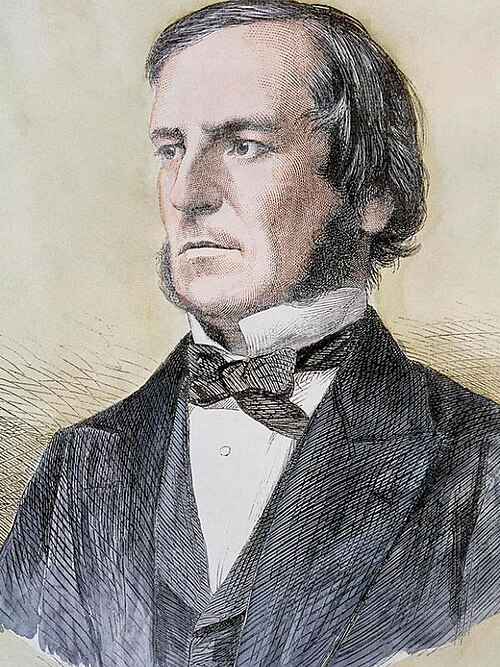
\includegraphics[width=0.28\textwidth]{boole.jpg}
  \caption{\textbf{George Boole (1815--1864)}, English mathematician and philosopher who formalized symbolic mathematical logic in \textit{The Laws of Thought} (1854), laying the algebraic foundation of modern computing and formal mathematics.}
  \label{fig:boole}
\end{figure}

\begin{definitionbox}{Elementary Logical Connectives}
Let $P$ and $Q$ be two propositions. We define compound propositions via truth functions:
\begin{enumerate}[leftmargin=1.4em,itemsep=3pt]
  \item \textbf{Negation ($\neg P$ or $\overline{P}$):} "Not $P$". True if and only if $P$ is false.
  \item \textbf{Conjunction ($P \land Q$):} "$P$ and $Q$". True if and only if both $P$ and $Q$ are simultaneously true.
  \item \textbf{Disjunction ($P \lor Q$):} "$P$ or $Q$" (inclusive or). True if at least one of $P$ or $Q$ is true; false only if both are false.
  \item \textbf{Implication ($P \implies Q$):} "$P$ implies $Q$" or "If $P$, then $Q$". False if and only if $P$ is true and $Q$ is false. By definition, $P \implies Q$ is logically equivalent to $(\neg P) \lor Q$.
  \item \textbf{Equivalence ($P \iff Q$):} "$P$ is equivalent to $Q$" or "$P$ if and only if $Q$". True if both $P$ and $Q$ possess the same truth value. Logically equivalent to $(P \implies Q) \land (Q \implies P)$.
\end{enumerate}
\end{definitionbox}

\begin{center}
\renewcommand{\arraystretch}{1.25}
\begin{tabular}{ccccccc}
\toprule
$P$ & $Q$ & $\neg P$ & $P \land Q$ & $P \lor Q$ & $P \implies Q$ & $P \iff Q$ \\
\midrule
$\mathrm{T}$ & $\mathrm{T}$ & $\mathrm{F}$ & $\mathrm{T}$ & $\mathrm{T}$ & $\mathrm{T}$ & $\mathrm{T}$ \\
$\mathrm{T}$ & $\mathrm{F}$ & $\mathrm{F}$ & $\mathrm{F}$ & $\mathrm{T}$ & $\mathrm{F}$ & $\mathrm{F}$ \\
$\mathrm{F}$ & $\mathrm{T}$ & $\mathrm{T}$ & $\mathrm{F}$ & $\mathrm{T}$ & $\mathrm{T}$ & $\mathrm{F}$ \\
$\mathrm{F}$ & $\mathrm{F}$ & $\mathrm{T}$ & $\mathrm{F}$ & $\mathrm{F}$ & $\mathrm{T}$ & $\mathrm{T}$ \\
\bottomrule
\end{tabular}
\end{center}

\begin{propbox}{Essential Tautologies and De Morgan's Logical Laws}
For any propositions $P, Q, R$, the following compound propositions are \textbf{tautologies} (true under all truth assignments):
\begin{enumerate}[leftmargin=1.4em,itemsep=2pt]
  \item \textbf{Double Negation:} $\neg(\neg P) \iff P$.
  \item \textbf{De Morgan's Laws:}
  \[
  \neg(P \land Q) \iff (\neg P) \lor (\neg Q), \qquad \neg(P \lor Q) \iff (\neg P) \land (\neg Q).
  \]
  \item \textbf{Distributivity:}
  \[
  P \land (Q \lor R) \iff (P \land Q) \lor (P \land R), \qquad P \lor (Q \land R) \iff (P \lor Q) \land (P \lor R).
  \]
  \item \textbf{Contrapositive Equivalence (Transposition):}
  \[
  (P \implies Q) \iff (\neg Q \implies \neg P).
  \]
  \item \textbf{Reductio ad Absurdum (Contradiction):}
  \[
  (P \implies Q) \iff \left[ (P \land \neg Q) \implies \text{Contradiction} \right].
  \]
\end{enumerate}
\end{propbox}

\section{Universal and Existential Quantifiers}

In mathematical analysis, assertions typically contain variables evaluated over specified sets. A statement containing a variable $x \in E$ is called an \textbf{open sentence} or \textbf{predicate}, denoted $P(x)$.

\begin{definitionbox}{Quantifiers and Their Scopes}
\begin{enumerate}[leftmargin=1.4em,itemsep=3pt]
  \item \textbf{Universal Quantifier ($\forall$, "for all" / "for every"):}
  \[
  \forall x \in E, \quad P(x)
  \]
  is true if and only if $P(x)$ holds true for every single element $x$ in the domain $E$.
  \item \textbf{Existential Quantifier ($\exists$, "there exists at least one"):}
  \[
  \exists x \in E, \quad P(x)
  \]
  is true if and only if there is at least one element $x \in E$ for which $P(x)$ is true.
  \item \textbf{Uniqueness Quantifier ($\exists!$, "there exists a unique"):}
  \[
  \exists! x \in E, \quad P(x) \iff \left[ (\exists x \in E, P(x)) \land (\forall x, y \in E, (P(x) \land P(y)) \implies x = y) \right].
  \]
\end{enumerate}
\end{definitionbox}

\begin{theorembox}{Negation of Quantified Statements}
The negation of quantified statements swaps the quantifiers and negates the inner predicate:
\begin{align}
\neg \left( \forall x \in E, \ P(x) \right) &\iff \exists x \in E, \ \neg P(x), \\
\neg \left( \exists x \in E, \ P(x) \right) &\iff \forall x \in E, \ \neg P(x).
\end{align}
For multi-quantifier propositions, the order of quantifiers is critical and cannot be arbitrarily exchanged:
\[
\exists y \in F, \ \forall x \in E, \ P(x, y) \implies \forall x \in E, \ \exists y \in F, \ P(x, y),
\]
but the converse is \textbf{false} in general!
\end{theorembox}

\section{Methods of Mathematical Proof}

\begin{enumerate}[leftmargin=1.4em,itemsep=4pt]
  \item \textbf{Direct Proof:} Assume $P$ is true. Through a sequence of rigorous deductions using axioms, definitions, and established theorems, show that $Q$ necessarily follows.
  \item \textbf{Proof by Contrapositive:} To prove $P \implies Q$, we prove the logically equivalent contrapositive statement $\neg Q \implies \neg P$. This is especially powerful when $\neg Q$ provides more concrete algebraic structure than $P$.
  \item \textbf{Proof by Contradiction (\textit{Reductio ad Absurdum}):} To prove an assertion $A$, assume its negation $\neg A$ is true. Derive a logical contradiction (such as $0 = 1$ or $x \in B \land x \notin B$). Therefore, $\neg A$ must be false, establishing that $A$ is true.
  \item \textbf{Disproof by Counterexample:} To disprove a universal assertion $\forall x \in E, P(x)$, it suffices to produce a single concrete element $x_0 \in E$ for which $P(x_0)$ is false.
  \item \textbf{Proof by Mathematical Induction:}
  \begin{theorembox}{Principle of Mathematical Induction (Peano Axiom)}
  Let $P(n)$ be a predicate defined for all integers $n \ge n_0$ ($n_0 \in \mathbb{Z}$). If:
  \begin{enumerate}[leftmargin=1.2em,itemsep=2pt]
    \item \textbf{Base Step:} $P(n_0)$ is true;
    \item \textbf{Inductive Step:} For any arbitrary integer $k \ge n_0$, the assumption that $P(k)$ is true (the \textit{induction hypothesis}) implies that $P(k+1)$ is true:
    \[
    \forall k \ge n_0, \quad P(k) \implies P(k+1);
    \]
  \end{enumerate}
  Then $P(n)$ is true for all integers $n \ge n_0$.
  \end{theorembox}
\end{enumerate}

\section{Axiomatic Set Theory and Operations}

A \textbf{set} is an intuitive collection of well-defined, distinct mathematical objects called its \textbf{elements}. If an object $x$ belongs to a set $A$, we write $x \in A$; otherwise $x \notin A$.

\begin{definitionbox}{Subsets, Equality, and the Power Set}
Let $A$ and $B$ be sets in a universe $E$:
\begin{enumerate}[leftmargin=1.4em,itemsep=2pt]
  \item \textbf{Inclusion (Subset):} $A \subseteq B \iff \forall x, (x \in A \implies x \in B)$.
  \item \textbf{Set Equality (Double Inclusion):} $A = B \iff (A \subseteq B \land B \subseteq A)$.
  \item \textbf{Empty Set ($\emptyset$):} The unique set containing no elements. For every set $A$, $\emptyset \subseteq A$.
  \item \textbf{Power Set ($\mathcal{P}(E)$):} The set of all subsets of $E$:
  \[
  \mathcal{P}(E) = \{ A \mid A \subseteq E \}.
  \]
  If $E$ is finite with $|E| = n$ elements, its power set has $|\mathcal{P}(E)| = 2^n$ elements.
\end{enumerate}
\end{definitionbox}

\begin{figure}[htbp]
  \centering
  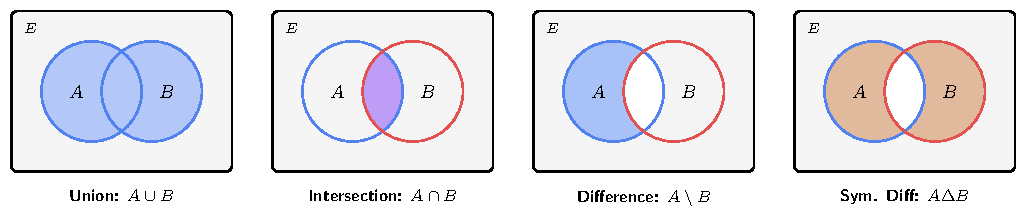
\includegraphics[width=0.95\textwidth]{01_venn_operations.pdf}
  \caption{\textbf{Fundamental Set Operations:} Geometric Venn diagram representation of Union ($A \cup B$), Intersection ($A \cap B$), Difference ($A \setminus B$), and Symmetric Difference ($A \Delta B$).}
  \label{fig:venn}
\end{figure}

\begin{definitionbox}{Fundamental Set Operations}
Let $A, B \in \mathcal{P}(E)$ be subsets of an ambient set $E$:
\begin{enumerate}[leftmargin=1.4em,itemsep=3pt]
  \item \textbf{Union:} $A \cup B = \{ x \in E \mid x \in A \lor x \in B \}$.
  \item \textbf{Intersection:} $A \cap B = \{ x \in E \mid x \in A \land x \in B \}$. If $A \cap B = \emptyset$, $A$ and $B$ are \textbf{disjoint}.
  \item \textbf{Set Difference (Relative Complement):} $A \setminus B = \{ x \in E \mid x \in A \land x \notin B \}$.
  \item \textbf{Complement in $E$:} $\complement_E A = E \setminus A = \{ x \in E \mid x \notin A \}$.
  \item \textbf{Symmetric Difference:} $A \Delta B = (A \setminus B) \cup (B \setminus A) = (A \cup B) \setminus (A \cap B)$.
  \item \textbf{Cartesian Product:} $A \times B = \{ (a, b) \mid a \in A \land b \in B \}$.
\end{enumerate}
\end{definitionbox}

\begin{theorembox}{De Morgan's Laws for Sets}
For any subsets $A, B \subseteq E$:
\begin{equation}
\complement_E (A \cup B) = \complement_E A \cap \complement_E B, \qquad \complement_E (A \cap B) = \complement_E A \cup \complement_E B.
\end{equation}
More generally, for any indexed family of subsets $\{A_i\}_{i \in I}$:
\begin{equation}
\complement_E \left( \bigcup_{i \in I} A_i \right) = \bigcap_{i \in I} \complement_E A_i, \qquad 
\complement_E \left( \bigcap_{i \in I} A_i \right) = \bigcup_{i \in I} \complement_E A_i.
\end{equation}
\end{theorembox}

\section{Worked Examples with Step-by-Step Proofs}

\begin{workedexample}{Irrationality of $\sqrt{2}$ by Contradiction}
Prove by contradiction that $\sqrt{2}$ is not a rational number ($\sqrt{2} \notin \mathbb{Q}$).

\paragraph{Solution and Proof.}
Assume to the contrary that the negation is true: $\sqrt{2} \in \mathbb{Q}$.
By definition of the rational numbers $\mathbb{Q}$, there exist two integers $a, b \in \mathbb{Z}$ with $b \neq 0$ such that:
\[
\sqrt{2} = \frac{a}{b}.
\]
Without loss of generality, we assume the fraction is in \textbf{irreducible form}, meaning that $\gcd(a, b) = 1$ ($a$ and $b$ share no common positive divisor other than $1$).

Squaring both sides of the equation:
\[
2 = \frac{a^2}{b^2} \implies a^2 = 2 b^2.
\]
This equation implies that $a^2$ is an even integer (a multiple of $2$).
\begin{itemize}[leftmargin=1.4em,itemsep=2pt]
  \item \textit{Lemma:} If $a^2$ is even, then $a$ is even.
  \item \textit{Proof of Lemma by Contrapositive:} Suppose $a$ is odd. Then $a = 2k + 1$ for some $k \in \mathbb{Z}$.
  Squaring gives $a^2 = (2k+1)^2 = 4k^2 + 4k + 1 = 2(2k^2 + 2k) + 1$, which is odd. Since the contrapositive holds, the lemma is established.
\end{itemize}
Because $a$ is even, there exists an integer $k \in \mathbb{Z}$ such that $a = 2k$.
Substituting $a = 2k$ back into our equation $a^2 = 2 b^2$:
\[
(2k)^2 = 2 b^2 \implies 4k^2 = 2 b^2 \implies b^2 = 2k^2.
\]
By the exact same reasoning, $b^2$ is even, which implies that $b$ must also be an even integer.

We have thus deduced that \textbf{both $a$ and $b$ are even}, meaning that $2$ divides both $a$ and $b$ ($2 \mid \gcd(a, b)$).
This directly contradicts our initial hypothesis that $\gcd(a, b) = 1$.
Therefore, the initial assumption that $\sqrt{2} \in \mathbb{Q}$ is false, concluding the proof that:
\[
\mathbf{\sqrt{2} \notin \mathbb{Q}}. \quad \blacksquare
\]
\end{workedexample}

\begin{workedexample}{Proof by Induction: Sum of the First $n$ Cubes}
Prove by mathematical induction that for every positive integer $n \ge 1$:
\[
\sum_{k=1}^n k^3 = 1^3 + 2^3 + 3^3 + \dots + n^3 = \left[ \frac{n(n+1)}{2} \right]^2.
\]

\paragraph{Solution and Proof.}
Let $P(n)$ be the proposition: $\sum_{k=1}^n k^3 = \left[ \frac{n(n+1)}{2} \right]^2$.

\textbf{1. Base Step ($n = 1$):}
For $n = 1$:
\[
\text{Left-Hand Side (LHS)} = 1^3 = 1.
\]
\[
\text{Right-Hand Side (RHS)} = \left[ \frac{1(1+1)}{2} \right]^2 = \left[ \frac{2}{2} \right]^2 = 1^2 = 1.
\]
Since $\mathrm{LHS} = \mathrm{RHS} = 1$, $P(1)$ is true.

\textbf{2. Inductive Step:}
Let $m \ge 1$ be an arbitrary integer. Assume that $P(m)$ is true (Induction Hypothesis):
\[
\sum_{k=1}^m k^3 = \left[ \frac{m(m+1)}{2} \right]^2.
\]
We must show that $P(m+1)$ is true, namely:
\[
\sum_{k=1}^{m+1} k^3 = \left[ \frac{(m+1)(m+2)}{2} \right]^2.
\]
Starting from the definition of the sum of $m+1$ terms:
\[
\sum_{k=1}^{m+1} k^3 = \left( \sum_{k=1}^m k^3 \right) + (m+1)^3.
\]
Substituting the Induction Hypothesis:
\[
\sum_{k=1}^{m+1} k^3 = \left[ \frac{m(m+1)}{2} \right]^2 + (m+1)^3 = \frac{m^2 (m+1)^2}{4} + (m+1)^3.
\]
Factoring out the common factor $(m+1)^2$:
\begin{align*}
\sum_{k=1}^{m+1} k^3 &= (m+1)^2 \left[ \frac{m^2}{4} + (m+1) \right] = (m+1)^2 \left[ \frac{m^2 + 4m + 4}{4} \right] \\
                    &= (m+1)^2 \left[ \frac{(m+2)^2}{4} \right] = \left[ \frac{(m+1)(m+2)}{2} \right]^2.
\end{align*}
This is precisely the statement $P(m+1)$.

\textbf{3. Conclusion:}
By the Principle of Mathematical Induction, the identity holds for all integers $n \ge 1$:
\[
\mathbf{\sum_{k=1}^n k^3 = \left[ \frac{n(n+1)}{2} \right]^2 = \left( \sum_{k=1}^n k \right)^2}. \quad \blacksquare
\]
\end{workedexample}

\begin{workedexample}{Rigorous Proof of De Morgan's Law for Sets}
Let $A$ and $B$ be two subsets of a universal set $E$. Prove rigorously by double inclusion that:
\[
\complement_E (A \cap B) = \complement_E A \cup \complement_E B.
\]

\paragraph{Solution and Proof.}
To establish set equality, we must prove two inclusions:
\begin{enumerate}[leftmargin=1.4em,itemsep=3pt]
  \item \textbf{Inclusion 1: $\complement_E (A \cap B) \subseteq \complement_E A \cup \complement_E B$.}
  Let $x \in \complement_E (A \cap B)$ be an arbitrary element.
  By definition of set complement:
  \[
  x \in E \quad \text{and} \quad x \notin (A \cap B).
  \]
  The statement $x \notin (A \cap B)$ is the logical negation of $x \in (A \cap B)$:
  \[
  \neg (x \in A \land x \in B).
  \]
  Applying De Morgan's logical law for conjunction:
  \[
  \neg (x \in A) \lor \neg (x \in B) \iff (x \notin A) \lor (x \notin B).
  \]
  Since $x \in E$, this translates to:
  \[
  (x \in E \land x \notin A) \lor (x \in E \land x \notin B) \iff x \in \complement_E A \lor x \in \complement_E B.
  \]
  By definition of set union:
  \[
  x \in (\complement_E A \cup \complement_E B).
  \]
  Since this holds for every $x \in \complement_E (A \cap B)$, we have established:
  \[
  \complement_E (A \cap B) \subseteq \complement_E A \cup \complement_E B.
  \]

  \item \textbf{Inclusion 2: $\complement_E A \cup \complement_E B \subseteq \complement_E (A \cap B)$.}
  Let $y \in (\complement_E A \cup \complement_E B)$ be an arbitrary element.
  By definition of union:
  \[
  y \in \complement_E A \lor y \in \complement_E B \iff (y \in E \land y \notin A) \lor (y \in E \land y \notin B).
  \]
  Thus $y \in E$ and $(y \notin A \lor y \notin B)$.
  By De Morgan's logical law, $(y \notin A \lor y \notin B) \iff \neg(y \in A \land y \in B) \iff y \notin (A \cap B)$.
  Therefore:
  \[
  y \in E \quad \text{and} \quad y \notin (A \cap B) \implies y \in \complement_E (A \cap B).
  \]
  This establishes the reverse inclusion:
  \[
  \complement_E A \cup \complement_E B \subseteq \complement_E (A \cap B).
  \]
\end{enumerate}
Combining both inclusions proves the identity:
\[
\mathbf{\complement_E (A \cap B) = \complement_E A \cup \complement_E B}. \quad \blacksquare
\]
\end{workedexample}

\begin{workedexample}{Characteristic Functions and Set Algebra}
For any subset $A \subseteq E$, its \textbf{characteristic function} (or indicator) is defined as:
\[
\mathbf{1}_A : E \longrightarrow \{0, 1\}, \qquad \mathbf{1}_A(x) = \begin{cases} 1 & \text{if } x \in A, \\ 0 & \text{if } x \notin A. \end{cases}
\]
\begin{enumerate}[leftmargin=1.4em,itemsep=2pt]
  \item Prove that for any two subsets $A, B \subseteq E$:
  \[
  \mathbf{1}_{A \cap B} = \mathbf{1}_A \cdot \mathbf{1}_B, \qquad \mathbf{1}_{\complement_E A} = 1 - \mathbf{1}_A.
  \]
  \item Using characteristic functions, derive the formula for the symmetric difference $\mathbf{1}_{A \Delta B}$.
\end{enumerate}

\paragraph{Solution and Proof.}
\textbf{1. Intersection and Complement:}
\begin{itemize}[leftmargin=1.4em,itemsep=2pt]
  \item For intersection: An element $x \in A \cap B \iff (x \in A \land x \in B)$.
  Thus $\mathbf{1}_{A \cap B}(x) = 1 \iff \mathbf{1}_A(x) = 1 \land \mathbf{1}_B(x) = 1 \iff \mathbf{1}_A(x) \cdot \mathbf{1}_B(x) = 1 \times 1 = 1$.
  If $x \notin A \cap B$, at least one of $\mathbf{1}_A(x)$ or $\mathbf{1}_B(x)$ is $0$, making the product $0$.
  Thus $\mathbf{1}_{A \cap B} = \mathbf{1}_A \cdot \mathbf{1}_B$.
  \item For complement: If $x \in \complement_E A$, then $x \notin A \implies \mathbf{1}_A(x) = 0$, so $1 - \mathbf{1}_A(x) = 1 - 0 = 1 = \mathbf{1}_{\complement_E A}(x)$.
  If $x \in A$, then $\mathbf{1}_A(x) = 1$, so $1 - \mathbf{1}_A(x) = 1 - 1 = 0 = \mathbf{1}_{\complement_E A}(x)$.
  Thus $\mathbf{1}_{\complement_E A} = 1 - \mathbf{1}_A$.
\end{itemize}

\textbf{2. Symmetric Difference $\mathbf{1}_{A \Delta B}$:}
Recall that $A \Delta B = (A \setminus B) \cup (B \setminus A) = (A \cap \complement_E B) \cup (B \cap \complement_E A)$.
Notice that $A \cap \complement_E B$ and $B \cap \complement_E A$ are strictly disjoint sets.
For any two disjoint sets $X$ and $Y$ ($X \cap Y = \emptyset$), $\mathbf{1}_{X \cup Y} = \mathbf{1}_X + \mathbf{1}_Y$.
Therefore:
\begin{align*}
\mathbf{1}_{A \Delta B} &= \mathbf{1}_{A \cap \complement_E B} + \mathbf{1}_{B \cap \complement_E A} \\
                       &= \mathbf{1}_A \cdot \mathbf{1}_{\complement_E B} + \mathbf{1}_B \cdot \mathbf{1}_{\complement_E A} \\
                       &= \mathbf{1}_A(1 - \mathbf{1}_B) + \mathbf{1}_B(1 - \mathbf{1}_A) \\
                       &= \mathbf{1}_A - \mathbf{1}_A \mathbf{1}_B + \mathbf{1}_B - \mathbf{1}_A \mathbf{1}_B \\
                       &= \mathbf{\mathbf{1}_A + \mathbf{1}_B - 2 \mathbf{1}_A \mathbf{1}_B} = (\mathbf{1}_A - \mathbf{1}_B)^2.
\end{align*}
This remarkable algebraic correspondence transforms boolean set manipulations directly into standard polynomial arithmetic!
\end{workedexample}

\chapter{Binary Relations, Mappings \& Abstract Algebraic Structures}
\label{chap:relations_structures}

\section{Binary Relations and Equivalence Structures}

\begin{definitionbox}{Binary Relation and Fundamental Axiomatic Properties}
Let $E$ be a set. A \textbf{binary relation} $\mathcal{R}$ on $E$ is formally defined as a subset of the Cartesian product: $\mathcal{R} \subseteq E \times E$. We write $x \mathcal{R} y$ if and only if $(x, y) \in \mathcal{R}$.
\begin{enumerate}[leftmargin=1.4em,itemsep=3pt]
  \item \textbf{Reflexivity:} $\forall x \in E, \ x \mathcal{R} x$.
  \item \textbf{Symmetry:} $\forall x, y \in E, \ (x \mathcal{R} y \implies y \mathcal{R} x)$.
  \item \textbf{Antisymmetry:} $\forall x, y \in E, \ ((x \mathcal{R} y \land y \mathcal{R} x) \implies x = y)$.
  \item \textbf{Transitivity:} $\forall x, y, z \in E, \ ((x \mathcal{R} y \land y \mathcal{R} z) \implies x \mathcal{R} z)$.
\end{enumerate}
\end{definitionbox}

\begin{definitionbox}{Equivalence Relations and Quotient Sets}
A binary relation $\mathcal{R}$ is an \textbf{equivalence relation} if it is simultaneously \textbf{reflexive, symmetric, and transitive}.
\begin{enumerate}[leftmargin=1.4em,itemsep=2pt]
  \item The \textbf{equivalence class} of an element $x \in E$ is the set of all elements related to $x$:
  \[
  \mathrm{cl}(x) \equiv [x] = \{ y \in E \mid x \mathcal{R} y \}.
  \]
  \item The \textbf{quotient set} $E / \mathcal{R}$ is the set of all distinct equivalence classes:
  \[
  E / \mathcal{R} = \{ [x] \mid x \in E \}.
  \]
\end{enumerate}
\end{definitionbox}

\begin{theorembox}{Fundamental Theorem of Equivalence Relations (Partition Theorem)}
Let $\mathcal{R}$ be an equivalence relation on $E$.
\begin{enumerate}[leftmargin=1.4em,itemsep=2pt]
  \item Two equivalence classes are either identical or completely disjoint:
  \[
  \forall x, y \in E, \quad [x] = [y] \iff x \mathcal{R} y, \qquad [x] \cap [y] = \emptyset \iff \neg(x \mathcal{R} y).
  \]
  \item The quotient set $E / \mathcal{R}$ forms a \textbf{partition} of $E$: the classes are non-empty, pairwise disjoint, and their union recovers $E$:
  \[
  \bigcup_{[x] \in E/\mathcal{R}} [x] = E.
  \]
\end{enumerate}
\end{theorembox}

\section{Order Relations and Posets}

\begin{definitionbox}{Partial and Total Orders}
A binary relation $\le$ on $E$ is an \textbf{order relation} if it is \textbf{reflexive, antisymmetric, and transitive}. The pair $(E, \le)$ is called a \textbf{partially ordered set} (or \textit{poset}).
\begin{itemize}[leftmargin=1.4em,itemsep=2pt]
  \item \textbf{Total Order (Chain):} If every pair of elements is comparable:
  \[
  \forall x, y \in E, \quad (x \le y \lor y \le x).
  \]
  \item \textbf{Partial Order:} There exist elements $x, y \in E$ such that neither $x \le y$ nor $y \le x$ (e.g. set inclusion $\subseteq$ on $\mathcal{P}(E)$).
\end{itemize}
\end{definitionbox}

\section{Mappings, Functions, and Morphisms}

\begin{figure}[htbp]
  \centering
  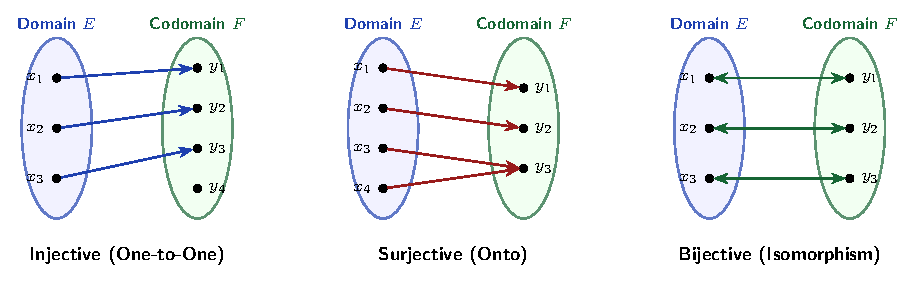
\includegraphics[width=0.95\textwidth]{02_mapping_types.pdf}
  \caption{\textbf{Classification of Mappings:} Injective (each codomain element has at most one preimage), Surjective (every codomain element has at least one preimage), and Bijective (exact one-to-one correspondence).}
  \label{fig:mappings}
\end{figure}

\begin{definitionbox}{Injectivity, Surjectivity, and Bijectivity}
Let $f: E \longrightarrow F$ be a mapping from set $E$ to set $F$:
\begin{enumerate}[leftmargin=1.4em,itemsep=3pt]
  \item \textbf{Injective (One-to-One):} Distinct domain elements map to distinct images:
  \[
  \forall x_1, x_2 \in E, \quad \left( f(x_1) = f(x_2) \implies x_1 = x_2 \right) \iff \left( x_1 \neq x_2 \implies f(x_1) \neq f(x_2) \right).
  \]
  \item \textbf{Surjective (Onto):} Every element of the codomain is the image of at least one domain element:
  \[
  \forall y \in F, \quad \exists x \in E \ \text{such that} \ f(x) = y \iff f(E) = F.
  \]
  \item \textbf{Bijective:} $f$ is both injective and surjective.
  Equivalently, for every $y \in F$, the equation $f(x) = y$ has a \textbf{unique solution} $x \in E$:
  \[
  \forall y \in F, \quad \exists! x \in E, \quad f(x) = y.
  \]
  A mapping $f$ is bijective if and only if there exists an inverse mapping $f^{-1}: F \longrightarrow E$ satisfying:
  \[
  f^{-1} \circ f = \mathrm{id}_E \quad \text{and} \quad f \circ f^{-1} = \mathrm{id}_F.
  \]
\end{enumerate}
\end{definitionbox}

\begin{propbox}{Properties of Image and Preimage Sets}
Let $f: E \longrightarrow F$. For any subsets $A, A' \subseteq E$ and $B, B' \subseteq F$:
\begin{enumerate}[leftmargin=1.4em,itemsep=2pt]
  \item $f(A \cup A') = f(A) \cup f(A')$ and $f(A \cap A') \subseteq f(A) \cap f(A')$ (equality holds if $f$ is injective).
  \item $f^{-1}(B \cup B') = f^{-1}(B) \cup f^{-1}(B')$ and $f^{-1}(B \cap B') = f^{-1}(B) \cap f^{-1}(B')$.
  \item $f^{-1}(\complement_F B) = \complement_E (f^{-1}(B))$. (Preimages preserve all boolean operations!).
\end{enumerate}
\end{propbox}

\section{Abstract Algebraic Structures}

\begin{figure}[htbp]
  \centering
  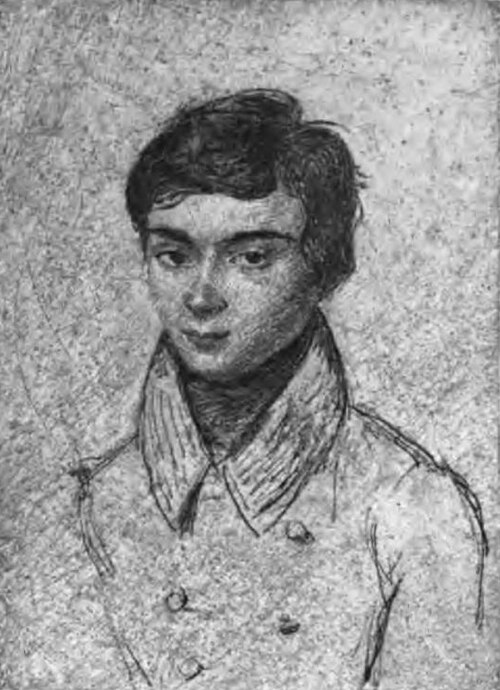
\includegraphics[width=0.28\textwidth]{galois.jpg}
  \caption{\textbf{Évariste Galois (1811--1832)}, French mathematical genius who introduced the concept of a \textit{group} and symmetry permutations to resolve the unsolvability of general quintic polynomial equations by radicals.}
  \label{fig:galois}
\end{figure}

\begin{definitionbox}{Groups, Subgroups, and Homomorphisms}
An \textbf{internal binary operation} on a set $G$ is a mapping $*: G \times G \longrightarrow G, (x, y) \mapsto x * y$.
\begin{enumerate}[leftmargin=1.4em,itemsep=3pt]
  \item A pair $(G, *)$ is a \textbf{Group} if:
  \begin{itemize}[leftmargin=1.2em,itemsep=1pt]
    \item \textbf{Associativity:} $\forall x, y, z \in G, \ (x * y) * z = x * (y * z)$.
    \item \textbf{Neutral Element:} $\exists e \in G, \ \forall x \in G, \ x * e = e * x = x$.
    \item \textbf{Invertibility:} $\forall x \in G, \ \exists x' \in G, \ x * x' = x' * x = e$ (denoted $x^{-1}$).
  \end{itemize}
  If additionally $\forall x, y \in G, x * y = y * x$, the group is \textbf{Abelian} (or commutative).
  \item \textbf{Subgroup Criterion:} A non-empty subset $H \subseteq G$ is a subgroup ($H \le G$) if and only if:
  \[
  \forall x, y \in H, \quad x * y^{-1} \in H.
  \]
  \item \textbf{Group Homomorphism:} A mapping $\phi: (G, *) \longrightarrow (G', \star)$ such that:
  \[
  \forall x, y \in G, \quad \phi(x * y) = \phi(x) \star \phi(y).
  \]
  The \textbf{kernel} $\ker(\phi) = \{ x \in G \mid \phi(x) = e' \}$ is a normal subgroup of $G$, and $\phi$ is injective if and only if $\ker(\phi) = \{ e \}$.
\end{enumerate}
\end{definitionbox}

\begin{definitionbox}{Rings and Fields}
\begin{enumerate}[leftmargin=1.4em,itemsep=3pt]
  \item A triplet $(A, +, \cdot)$ is a \textbf{Ring} if $(A, +)$ is an abelian group (neutral $0$), the operation $\cdot$ is associative, and $\cdot$ distributes over $+$:
  \[
  \forall x, y, z \in A, \quad x \cdot (y + z) = x \cdot y + x \cdot z \quad \text{and} \quad (y + z) \cdot x = y \cdot x + z \cdot x.
  \]
  \item A ring $(K, +, \cdot)$ is a \textbf{Field} (Corps) if $0 \neq 1$, multiplication is commutative, and every non-zero element $x \in K \setminus \{0\}$ has a multiplicative inverse $x^{-1}$.
  (\textit{Examples:} $\mathbb{Q}, \mathbb{R}, \mathbb{C}$ are fields; $\mathbb{Z}$ is an integral domain but not a field).
\end{enumerate}
\end{definitionbox}

\section{Worked Examples with Step-by-Step Proofs}

\begin{workedexample}{Modular Arithmetic as an Equivalence Relation}
Fix an integer $n \ge 2$. On the set of integers $\mathbb{Z}$, define the relation of \textbf{congruence modulo $n$} by:
\[
x \equiv y \pmod n \iff n \mid (x - y) \iff \exists k \in \mathbb{Z}, \ x - y = k n.
\]
\begin{enumerate}[leftmargin=1.4em,itemsep=2pt]
  \item Prove rigorously that $\equiv \pmod n$ is an equivalence relation on $\mathbb{Z}$.
  \item Describe explicitly the equivalence classes and the quotient set $\mathbb{Z} / n\mathbb{Z}$.
\end{enumerate}

\paragraph{Solution and Proof.}
\textbf{1. Verification of Equivalence Axioms:}
\begin{itemize}[leftmargin=1.4em,itemsep=2pt]
  \item \textbf{Reflexivity:} For any $x \in \mathbb{Z}$, $x - x = 0 = 0 \cdot n$. Since $0 \in \mathbb{Z}$, $n \mid (x - x)$, so $x \equiv x \pmod n$.
  \item \textbf{Symmetry:} Let $x, y \in \mathbb{Z}$ such that $x \equiv y \pmod n$.
  Then $x - y = k n$ for some $k \in \mathbb{Z}$. Multiplying by $-1$:
  \[
  y - x = -(x - y) = -k n = (-k) n.
  \]
  Since $-k \in \mathbb{Z}$, $n \mid (y - x)$, so $y \equiv x \pmod n$.
  \item \textbf{Transitivity:} Let $x, y, z \in \mathbb{Z}$ such that $x \equiv y \pmod n$ and $y \equiv z \pmod n$.
  Then $x - y = k_1 n$ and $y - z = k_2 n$ for integers $k_1, k_2 \in \mathbb{Z}$.
  Adding the two equations:
  \[
  (x - y) + (y - z) = k_1 n + k_2 n \implies x - z = (k_1 + k_2) n.
  \]
  Since $k_1 + k_2 \in \mathbb{Z}$, $n \mid (x - z)$, so $x \equiv z \pmod n$.
\end{itemize}
Therefore, $\equiv \pmod n$ is an equivalence relation.

\textbf{2. Equivalence Classes and Quotient Set:}
By the Euclidean division algorithm, for any integer $x \in \mathbb{Z}$, dividing by $n$ yields unique integers $q \in \mathbb{Z}$ and $r \in \{0, 1, 2, \dots, n-1\}$ such that:
\[
x = q n + r \implies x - r = q n \implies x \equiv r \pmod n.
\]
Hence, every integer belongs to the equivalence class of its remainder $r \in \{0, 1, \dots, n-1\}$:
\[
[r] = \{ r + k n \mid k \in \mathbb{Z} \} = r + n\mathbb{Z}.
\]
The quotient set consists of exactly $n$ distinct equivalence classes:
\[
\mathbf{\mathbb{Z} / n\mathbb{Z} = \{ [0], [1], [2], \dots, [n-1] \}}. \quad \blacksquare
\]
\end{workedexample}

\begin{workedexample}{Injectivity, Surjectivity, and Bijectivity Verification}
Consider the mapping:
\[
f: \mathbb{R} \setminus \{2\} \longrightarrow \mathbb{R} \setminus \{1\}, \qquad f(x) = \frac{x + 1}{x - 2}.
\]
\begin{enumerate}[leftmargin=1.4em,itemsep=2pt]
  \item Prove from first principles that $f$ is injective.
  \item Prove from first principles that $f$ is surjective.
  \item Deduce that $f$ is bijective and determine its explicit inverse mapping $f^{-1}(y)$.
\end{enumerate}

\paragraph{Solution and Proof.}
\textbf{1. Proof of Injectivity:}
Let $x_1, x_2 \in \mathbb{R} \setminus \{2\}$ such that $f(x_1) = f(x_2)$:
\[
\frac{x_1 + 1}{x_1 - 2} = \frac{x_2 + 1}{x_2 - 2}.
\]
Cross-multiplying denominators:
\[
(x_1 + 1)(x_2 - 2) = (x_2 + 1)(x_1 - 2).
\]
Expanding both products:
\[
x_1 x_2 - 2 x_1 + x_2 - 2 = x_1 x_2 - 2 x_2 + x_1 - 2.
\]
Subtracting the common terms $x_1 x_2 - 2$ from both sides:
\[
-2 x_1 + x_2 = -2 x_2 + x_1 \implies 3 x_2 = 3 x_1 \implies x_1 = x_2.
\]
Thus $f$ is strictly \textbf{injective}.

\textbf{2. Proof of Surjectivity:}
Let $y \in \mathbb{R} \setminus \{1\}$ be an arbitrary element of the codomain. We must find $x \in \mathbb{R} \setminus \{2\}$ such that $f(x) = y$:
\[
\frac{x + 1}{x - 2} = y \implies x + 1 = y(x - 2) = y x - 2y.
\]
Isolating terms in $x$:
\[
1 + 2y = y x - x = x(y - 1).
\]
Since $y \neq 1$, we can divide by $(y - 1) \neq 0$:
\[
x = \frac{2y + 1}{y - 1}.
\]
We must verify that this candidate $x \neq 2$:
If $\frac{2y+1}{y-1} = 2 \implies 2y + 1 = 2y - 2 \implies 1 = -2$, which is impossible.
Hence $x \in \mathbb{R} \setminus \{2\}$ always exists and is well-defined.
Thus $f$ is \textbf{surjective}.

\textbf{3. Bijectivity and Inverse Mapping:}
Since $f$ is both injective and surjective, it is a \textbf{bijection}.
Its inverse mapping $f^{-1}: \mathbb{R} \setminus \{1\} \longrightarrow \mathbb{R} \setminus \{2\}$ is:
\[
\mathbf{f^{-1}(y) = \frac{2y + 1}{y - 1}}. \quad \blacksquare
\]
\end{workedexample}

\begin{workedexample}{Subgroup Verification and Matrix Groups}
Let $\mathrm{GL}_2(\mathbb{R})$ denote the general linear group of $2 \times 2$ invertible real matrices under matrix multiplication. Consider the subset:
\[
\mathrm{SL}_2(\mathbb{R}) = \{ M \in \mathrm{GL}_2(\mathbb{R}) \mid \det(M) = 1 \}.
\]
Prove using the subgroup criterion that $\mathrm{SL}_2(\mathbb{R})$ is a subgroup of $\mathrm{GL}_2(\mathbb{R})$ (the \textit{Special Linear Group}).

\paragraph{Solution and Proof.}
We verify the three conditions of the subgroup criterion:
\begin{enumerate}[leftmargin=1.4em,itemsep=3pt]
  \item \textbf{Non-emptiness:}
  The identity matrix $I_2 = \begin{pmatrix} 1 & 0 \\ 0 & 1 \end{pmatrix}$ has determinant:
  \[
  \det(I_2) = (1)(1) - (0)(0) = 1.
  \]
  Thus $I_2 \in \mathrm{SL}_2(\mathbb{R})$, establishing that $\mathrm{SL}_2(\mathbb{R}) \neq \emptyset$.
  \item \textbf{Closure under Inverse:}
  Let $A \in \mathrm{SL}_2(\mathbb{R})$. Then $\det(A) = 1 \neq 0$, so $A^{-1}$ exists in $\mathrm{GL}_2(\mathbb{R})$.
  By the multiplicative property of determinants:
  \[
  \det(A \cdot A^{-1}) = \det(I_2) = 1 \implies \det(A) \cdot \det(A^{-1}) = 1.
  \]
  Since $\det(A) = 1$, we have $1 \cdot \det(A^{-1}) = 1 \implies \det(A^{-1}) = 1$.
  Therefore, $A^{-1} \in \mathrm{SL}_2(\mathbb{R})$.
  \item \textbf{Closure under Product (Combined Criterion $A B^{-1} \in \mathrm{SL}_2(\mathbb{R})$):}
  Let $A, B \in \mathrm{SL}_2(\mathbb{R})$.
  \[
  \det(A B^{-1}) = \det(A) \cdot \det(B^{-1}) = 1 \times 1 = 1.
  \]
  Therefore, $A B^{-1} \in \mathrm{SL}_2(\mathbb{R})$.
\end{enumerate}
By the Subgroup Criterion, $\mathbf{\mathrm{SL}_2(\mathbb{R}) \le \mathrm{GL}_2(\mathbb{R})}$ is a subgroup. $\blacksquare$
\end{workedexample}

\begin{workedexample}{Kernel and Image of a Group Homomorphism}
Consider the mapping $\phi: (\mathbb{R}, +) \longrightarrow (\mathbb{C}^*, \cdot)$ defined by:
\[
\phi(x) = e^{i x} = \cos(x) + i \sin(x).
\]
\begin{enumerate}[leftmargin=1.4em,itemsep=2pt]
  \item Prove that $\phi$ is a group homomorphism.
  \item Determine the kernel $\ker(\phi)$ and describe its algebraic nature.
  \item Determine the image $\mathrm{Im}(\phi)$.
\end{enumerate}

\paragraph{Solution and Proof.}
\textbf{1. Proof of Homomorphism:}
For any $x, y \in \mathbb{R}$:
\[
\phi(x + y) = e^{i(x + y)} = e^{i x} \cdot e^{i y} = \phi(x) \cdot \phi(y).
\]
Since addition in the domain maps to multiplication in the codomain, $\phi$ is a group homomorphism.

\textbf{2. Kernel Determination:}
The neutral element of $(\mathbb{C}^*, \cdot)$ is $1$. By definition:
\[
\ker(\phi) = \{ x \in \mathbb{R} \mid \phi(x) = 1 \} = \{ x \in \mathbb{R} \mid \cos x + i \sin x = 1 \}.
\]
Equating real and imaginary parts:
\[
\cos x = 1 \quad \text{and} \quad \sin x = 0 \iff x = 2 k \pi \quad (k \in \mathbb{Z}).
\]
Therefore:
\[
\mathbf{\ker(\phi) = 2\pi\mathbb{Z} = \{ 2 k \pi \mid k \in \mathbb{Z} \}}.
\]
Notice that $\ker(\phi) \neq \{0\}$, proving that $\phi$ is \textbf{not injective}.

\textbf{3. Image Determination:}
For every $x \in \mathbb{R}$, $|\phi(x)| = |e^{i x}| = \sqrt{\cos^2 x + \sin^2 x} = 1$.
Every complex number on the unit circle $\mathbb{U} = \{ z \in \mathbb{C} \mid |z| = 1 \}$ can be written in polar form as $e^{i \theta}$ for some $\theta \in \mathbb{R}$.
Therefore:
\[
\mathbf{\mathrm{Im}(\phi) = \mathbb{U} \equiv \mathbb{S}^1} \quad \text{(the Circle Group)}. \quad \blacksquare
\]
\end{workedexample}

\chapter{The Real Number System ($\mathbb{R}$)}
\label{chap:real_numbers}

\section{Axiomatic Structure of the Real Field}

The set of real numbers $\mathbb{R}$ is axiomatically characterized as a **complete, Archimedean, totally ordered field**. While the rational numbers $\mathbb{Q}$ form an ordered field, they exhibit fatal topological "gaps" (such as $\sqrt{2} \notin \mathbb{Q}$ or $\pi \notin \mathbb{Q}$). The construction of $\mathbb{R}$ seals every gap through the **Completeness Axiom**.

\begin{figure}[htbp]
  \centering
  \begin{minipage}{0.35\textwidth}
    \centering
    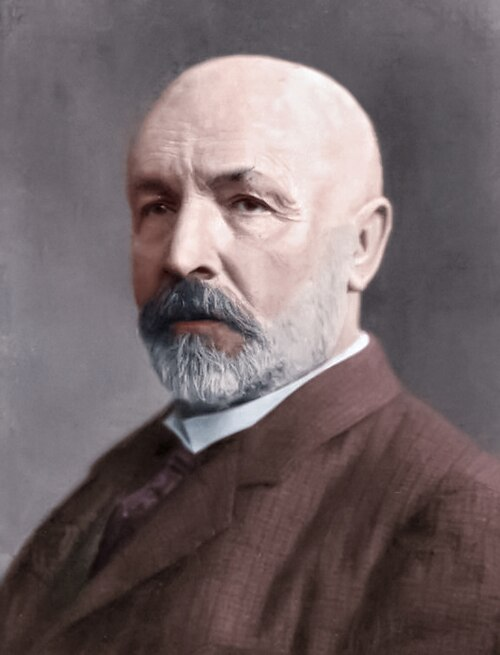
\includegraphics[width=0.82\textwidth]{cantor.jpg}
    \caption*{(a) \textbf{Georg Cantor (1845--1918)}}
  \end{minipage}
  \hspace{0.08\textwidth}
  \begin{minipage}{0.35\textwidth}
    \centering
    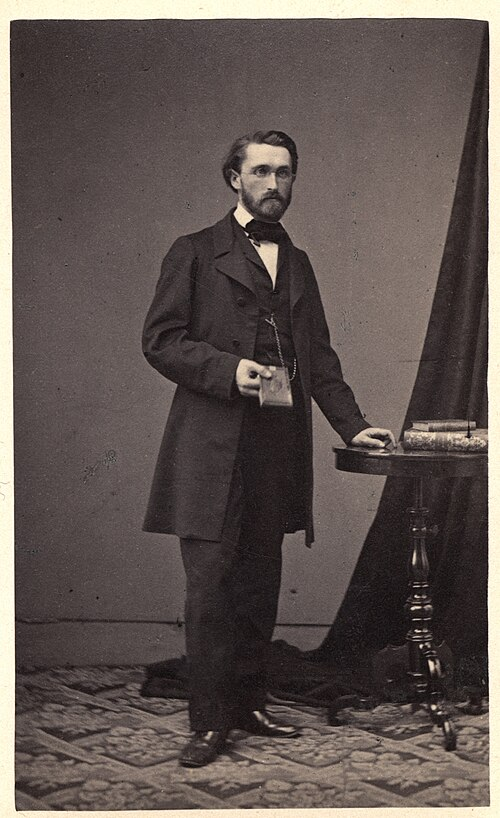
\includegraphics[width=0.82\textwidth]{dedekind.jpg}
    \caption*{(b) \textbf{Richard Dedekind (1831--1916)}}
  \end{minipage}
  \caption{\textbf{Founders of Real Analysis:} Georg Cantor (inventor of transfinite set theory and diagonal cardinality) and Richard Dedekind (creator of Dedekind cuts, providing the first rigorous construction of the real continuum $\mathbb{R}$ from $\mathbb{Q}$).}
  \label{fig:cantor_dedekind}
\end{figure}

\begin{definitionbox}{Absolute Value and Distance on $\mathbb{R}$}
For any real number $x \in \mathbb{R}$, its \textbf{absolute value} $|x|$ is defined by:
\[
|x| = \begin{cases} x & \text{if } x \ge 0, \\ -x & \text{if } x < 0. \end{cases} \iff |x| = \max(x, -x) = \sqrt{x^2}.
\]
The Euclidean distance between two numbers $x, y \in \mathbb{R}$ is $d(x, y) = |x - y|$.
\end{definitionbox}

\begin{theorembox}{The Triangle Inequalities}
For all real numbers $x, y \in \mathbb{R}$:
\begin{enumerate}[leftmargin=1.4em,itemsep=3pt]
  \item \textbf{Standard Triangle Inequality:}
  \[
  |x + y| \le |x| + |y|.
  \]
  Equality holds if and only if $x$ and $y$ have the same sign ($x y \ge 0$).
  \item \textbf{Reverse Triangle Inequality:}
  \[
  \big| |x| - |y| \big| \le |x - y|.
  \]
  \item \textbf{Generalized $n$-term Inequality:}
  \[
  \left| \sum_{k=1}^n x_k \right| \le \sum_{k=1}^n |x_k|.
  \]
\end{enumerate}
\end{theorembox}

\section{Bounded Sets, Maximum, Minimum, Supremum and Infimum}

\begin{definitionbox}{Upper Bounds, Lower Bounds, Extrema}
Let $A$ be a non-empty subset of $\mathbb{R}$ ($A \subseteq \mathbb{R}, A \neq \emptyset$):
\begin{enumerate}[leftmargin=1.4em,itemsep=3pt]
  \item \textbf{Bounded Above (Majoré):} $\exists M \in \mathbb{R}, \ \forall x \in A, \ x \le M$. $M$ is an \textbf{upper bound} (majorant).
  \item \textbf{Bounded Below (Minoré):} $\exists m \in \mathbb{R}, \ \forall x \in A, \ x \ge m$. $m$ is a \textbf{lower bound} (minorant).
  \item \textbf{Bounded Set (Borné):} $A$ is both bounded above and below:
  \[
  \exists K > 0, \quad \forall x \in A, \quad |x| \le K.
  \]
  \item \textbf{Maximum (Greatest Element):} An upper bound $M$ that \textbf{belongs to the set}:
  \[
  M = \max A \iff (M \in A \ \land \ \forall x \in A, x \le M).
  \]
  \item \textbf{Minimum (Least Element):} A lower bound $m$ that belongs to the set:
  \[
  m = \min A \iff (m \in A \ \land \ \forall x \in A, x \ge m).
  \]
\end{enumerate}
\end{definitionbox}

\begin{figure}[htbp]
  \centering
  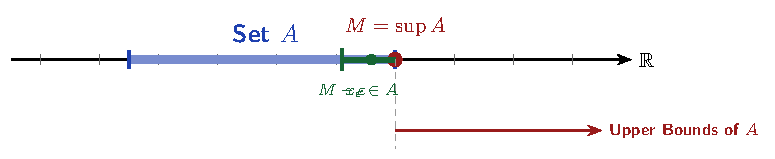
\includegraphics[width=0.88\textwidth]{03_real_completeness.pdf}
  \caption{\textbf{The Completeness Axiom and Supremum Characterization:} The supremum $M = \sup A$ is the least upper bound. For any arbitrary small $\varepsilon > 0$, the interval $(M - \varepsilon, M]$ contains at least one element $x_\varepsilon \in A$.}
  \label{fig:completeness}
\end{figure}

\begin{theorembox}{The Axiom of Completeness (Axiom of the Supremum)}
Every non-empty subset $A \subset \mathbb{R}$ that is bounded above possesses a \textbf{least upper bound} in $\mathbb{R}$, denoted $\sup A$ (\textbf{supremum} or \textit{borne supérieure}).

Similarly, every non-empty subset $A \subset \mathbb{R}$ that is bounded below possesses a \textbf{greatest lower bound} in $\mathbb{R}$, denoted $\inf A$ (\textbf{infimum} or \textit{borne inférieure}).
\end{theorembox}

\begin{propbox}{Analytical $\varepsilon$-Characterization of Supremum and Infimum}
Let $A \subset \mathbb{R}$ be non-empty and bounded above. A real number $S \in \mathbb{R}$ is the supremum ($S = \sup A$) if and only if:
\begin{equation}
\begin{cases}
(1) & \forall x \in A, \quad x \le S \quad (\text{$S$ is an upper bound}) \\
(2) & \forall \varepsilon > 0, \quad \exists x_\varepsilon \in A \ \text{such that} \ x_\varepsilon > S - \varepsilon \quad (\text{no smaller upper bound exists})
\end{cases}
\end{equation}
Similarly, $I = \inf A$ if and only if:
\begin{equation}
\begin{cases}
(1) & \forall x \in A, \quad x \ge I \quad (\text{$I$ is a lower bound}) \\
(2) & \forall \varepsilon > 0, \quad \exists x_\varepsilon \in A \ \text{such that} \ x_\varepsilon < I + \varepsilon
\end{cases}
\end{equation}
\end{propbox}

\section{The Archimedean Property and Density}

\begin{theorembox}{The Archimedean Property of $\mathbb{R}$}
The real number field $\mathbb{R}$ is \textbf{Archimedean}: it contains no infinitely large or infinitesimally small elements.
\begin{equation}
\forall x \in \mathbb{R}, \quad \exists n \in \mathbb{N} \quad \text{such that} \quad n > x.
\end{equation}
\textbf{Fundamental Analytical Equivalences:}
\begin{enumerate}[leftmargin=1.4em,itemsep=2pt]
  \item $\forall \varepsilon > 0, \ \exists n \in \mathbb{N}^* \ \text{such that} \ \frac{1}{n} < \varepsilon$.
  \item $\forall x, y \in \mathbb{R}$ with $x > 0$, $\exists n \in \mathbb{N}$ such that $n x > y$.
  \item The set of natural numbers $\mathbb{N}$ is not bounded above in $\mathbb{R}$ ($\sup \mathbb{N} = +\infty$).
\end{enumerate}
\end{theorembox}

\begin{propbox}{The Floor Function (Integer Part)}
For every real number $x \in \mathbb{R}$, there exists a **unique** integer $p \in \mathbb{Z}$ such that:
\begin{equation}
p \le x < p + 1.
\end{equation}
This integer is the \textbf{integer part} (or floor) of $x$, denoted $E(x) \equiv \lfloor x \rfloor = p$.
\end{propbox}

\begin{theorembox}{Density of Rational and Irrational Numbers in $\mathbb{R}$}
Between any two distinct real numbers, there exist infinitely many rational numbers and infinitely many irrational numbers:
\begin{equation}
\forall a, b \in \mathbb{R} \ \text{with} \ a < b, \quad \exists r \in \mathbb{Q} \ \text{and} \ \exists \alpha \in \mathbb{R} \setminus \mathbb{Q} \quad \text{such that} \quad a < r < \alpha < b.
\end{equation}
In topological terms, both $\mathbb{Q}$ and $\mathbb{R} \setminus \mathbb{Q}$ are \textbf{dense} in $\mathbb{R}$ ($\overline{\mathbb{Q}} = \mathbb{R}$ and $\overline{\mathbb{R} \setminus \mathbb{Q}} = \mathbb{R}$).
\end{theorembox}

\section{Worked Examples with Step-by-Step Proofs}

\begin{workedexample}{Rigorous Proof of the Archimedean Property from Completeness}
Prove rigorously that the Archimedean property ($\forall x \in \mathbb{R}, \exists n \in \mathbb{N}: n > x$) is a direct consequence of the Completeness Axiom of $\mathbb{R}$.

\paragraph{Solution and Proof.}
We proceed by contradiction (\textit{reductio ad absurdum}).
Assume that the Archimedean property is false. Then its logical negation is true:
\[
\exists x_0 \in \mathbb{R}, \quad \forall n \in \mathbb{N}, \quad n \le x_0.
\]
This statement asserts that $x_0$ is an \textbf{upper bound} for the set of natural numbers $\mathbb{N} \subset \mathbb{R}$.
Therefore, $\mathbb{N}$ is a non-empty subset of $\mathbb{R}$ bounded above by $x_0$.

By the \textbf{Completeness Axiom}, $\mathbb{N}$ must possess a supremum in $\mathbb{R}$:
\[
S = \sup \mathbb{N} \in \mathbb{R}.
\]
Now consider $\varepsilon = 1 > 0$.
By the $\varepsilon$-characterization of the supremum, $S - 1$ is strictly strictly smaller than $S$, so $S - 1$ \textbf{cannot be an upper bound} of $\mathbb{N}$.
Therefore, there exists at least one element $m \in \mathbb{N}$ such that:
\[
m > S - 1.
\]
Adding $1$ to both sides of this inequality:
\[
m + 1 > S.
\]
Since $m \in \mathbb{N}$, its successor $m + 1$ is also a natural number ($m + 1 \in \mathbb{N}$).
Thus, we have found an element of $\mathbb{N}$ that is strictly strictly greater than $S = \sup \mathbb{N}$.
This contradicts the fundamental definition of $S$ as an upper bound of $\mathbb{N}$!

Therefore, the assumption is impossible, establishing that:
\[
\mathbf{\forall x \in \mathbb{R}, \quad \exists n \in \mathbb{N} \quad \text{such that} \quad n > x}. \quad \blacksquare
\]
\end{workedexample}

\begin{workedexample}{Determining $\sup, \inf, \max, \min$ of a Real Set}
Consider the set:
\[
A = \left\{ \frac{2n - 1}{n + 2} \;\middle|\; n \in \mathbb{N}^* \right\} = \left\{ \frac{1}{3}, \frac{3}{4}, \frac{5}{5}, \frac{7}{6}, \dots \right\}.
\]
\begin{enumerate}[leftmargin=1.4em,itemsep=2pt]
  \item Determine $\min A$ and $\inf A$, proving your answer rigorously.
  \item Prove that $A$ has no maximum ($\max A$ does not exist).
  \item Determine $\sup A$ using the $\varepsilon$-characterization property.
\end{enumerate}

\paragraph{Solution and Proof.}
Rewrite the general element $x_n = \frac{2n - 1}{n + 2}$ by polynomial division:
\[
x_n = \frac{2(n + 2) - 5}{n + 2} = 2 - \frac{5}{n + 2}.
\]
\textbf{1. Infimum and Minimum:}
As $n$ increases ($n \in \{1, 2, 3, \dots\}$), the denominator $n+2$ increases, so $\frac{5}{n+2}$ strictly decreases.
Therefore, $x_n = 2 - \frac{5}{n+2}$ is a \textbf{strictly increasing sequence}:
\[
x_1 = 2 - \frac{5}{3} = \frac{1}{3}, \quad x_2 = 2 - \frac{5}{4} = \frac{3}{4}, \quad \dots
\]
For all $n \ge 1$:
\[
x_n \ge x_1 = \frac{1}{3}.
\]
Thus $1/3$ is a lower bound of $A$. Moreover, since $1/3 = x_1 \in A$:
\[
\mathbf{\min A = \inf A = \frac{1}{3}}.
\]

\textbf{2. Non-existence of Maximum:}
Since $n+2 > 0$ for all $n \ge 1$, $\frac{5}{n+2} > 0$, which means:
\[
x_n = 2 - \frac{5}{n+2} < 2 \quad \text{for all } n \in \mathbb{N}^*.
\]
Thus $2$ is an upper bound of $A$, but $2 \notin A$ (since $2 - \frac{5}{n+2} = 2 \implies \frac{5}{n+2} = 0$, which has no real solution).
Because the sequence $x_n$ is strictly increasing, every element $x_n$ is strictly smaller than $x_{n+1} \in A$.
Therefore, no single element in $A$ can be the greatest element: $\mathbf{\max A \text{ does not exist}}$.

\textbf{3. Supremum Determination via $\varepsilon$-Characterization:}
We claim that $\sup A = 2$.
\begin{itemize}[leftmargin=1.4em,itemsep=2pt]
  \item \textbf{Condition 1 (Upper Bound):} We already showed $\forall n \ge 1, x_n < 2$. Thus $2$ is an upper bound.
  \item \textbf{Condition 2 ($\varepsilon$-Condition):} Let $\varepsilon > 0$ be given. We must find an integer $n \in \mathbb{N}^*$ such that:
  \[
  x_n > 2 - \varepsilon \iff 2 - \frac{5}{n + 2} > 2 - \varepsilon \iff \frac{5}{n + 2} < \varepsilon \iff n + 2 > \frac{5}{\varepsilon} \iff n > \frac{5}{\varepsilon} - 2.
  \]
  By the Archimedean property of $\mathbb{R}$, there always exists an integer $n_0 \in \mathbb{N}^*$ such that $n_0 > \frac{5}{\varepsilon} - 2$.
  Choosing this $n_0$, we have $x_{n_0} \in A$ and $x_{n_0} > 2 - \varepsilon$.
\end{itemize}
Both conditions of the $\varepsilon$-characterization are satisfied. Therefore:
\[
\mathbf{\sup A = 2}. \quad \blacksquare
\]
\end{workedexample}

\begin{workedexample}{Density Proof: Constructing a Rational Between Any Two Reals}
Prove rigorously that for any real numbers $x, y \in \mathbb{R}$ with $x < y$, there exists a rational number $r \in \mathbb{Q}$ such that:
\[
x < r < y.
\]

\paragraph{Solution and Proof.}
Since $x < y$, the interval length is strictly positive: $y - x > 0$.
\begin{enumerate}[leftmargin=1.4em,itemsep=3pt]
  \item \textbf{Choice of Denominator $n$:}
  By the Archimedean property, there exists an integer $n \in \mathbb{N}^*$ such that:
  \[
  n > \frac{1}{y - x} \iff \frac{1}{n} < y - x \iff n y - n x > 1.
  \]
  \item \textbf{Choice of Numerator $m$:}
  Consider the number $n x$. By the floor function property, there exists a unique integer $m \in \mathbb{Z}$ such that:
  \[
  m - 1 \le n x < m \iff n x < m \le n x + 1.
  \]
  \item \textbf{Verification of Inequalities:}
  From the left inequality:
  \[
  n x < m \implies x < \frac{m}{n}.
  \]
  From the right inequality and since $n y - n x > 1 \implies n x + 1 < n y$:
  \[
  m \le n x + 1 < n y \implies m < n y \implies \frac{m}{n} < y.
  \]
  Combining both inequalities:
  \[
  x < \frac{m}{n} < y.
  \]
\end{enumerate}
Setting $r = \frac{m}{n} \in \mathbb{Q}$, we have established that $\mathbf{x < r < y}$. $\blacksquare$
\end{workedexample}

\begin{workedexample}{Supremum of a Two-Variable Bounded Set}
Let $A$ and $B$ be two non-empty subsets of $\mathbb{R}$ bounded above. Define:
\[
A + B = \{ x + y \mid x \in A \land y \in B \}.
\]
Prove that $A + B$ is bounded above and that:
\[
\sup(A + B) = \sup A + \sup B.
\]

\paragraph{Solution and Proof.}
Let $S_A = \sup A$ and $S_B = \sup B$.
\begin{enumerate}[leftmargin=1.4em,itemsep=3pt]
  \item \textbf{$S_A + S_B$ is an Upper Bound for $A + B$:}
  Let $z \in A + B$. By definition, $z = x + y$ with $x \in A$ and $y \in B$.
  Since $S_A$ is an upper bound of $A$, $x \le S_A$.
  Since $S_B$ is an upper bound of $B$, $y \le S_B$.
  Adding the two inequalities:
  \[
  z = x + y \le S_A + S_B.
  \]
  Since this holds for every $z \in A + B$, $A + B$ is bounded above by $S_A + S_B$.
  By the Completeness Axiom, $\sup(A + B)$ exists, and:
  \[
  \sup(A + B) \le S_A + S_B.
  \]

  \item \textbf{Reverse Inequality via $\varepsilon$-Characterization:}
  Let $\varepsilon > 0$ be given. Consider $\varepsilon' = \frac{\varepsilon}{2} > 0$.
  \begin{itemize}[leftmargin=1.4em,itemsep=2pt]
    \item By the $\varepsilon$-characterization of $\sup A$, there exists $x_0 \in A$ such that $x_0 > S_A - \frac{\varepsilon}{2}$.
    \item By the $\varepsilon$-characterization of $\sup B$, there exists $y_0 \in B$ such that $y_0 > S_B - \frac{\varepsilon}{2}$.
  \end{itemize}
  Adding these two inequalities:
  \[
  x_0 + y_0 > \left( S_A - \frac{\varepsilon}{2} \right) + \left( S_B - \frac{\varepsilon}{2} \right) = (S_A + S_B) - \varepsilon.
  \]
  Since $x_0 + y_0 \in A + B$, we have found an element of $A + B$ strictly greater than $(S_A + S_B) - \varepsilon$.
  Therefore, no number strictly smaller than $S_A + S_B$ can be an upper bound for $A + B$.
  This proves that:
  \[
  \sup(A + B) \ge S_A + S_B.
  \]
\end{enumerate}
Combining both inequalities yields the exact equality:
\[
\mathbf{\sup(A + B) = \sup A + \sup B}. \quad \blacksquare
\]
\end{workedexample}

\chapter{Numerical Sequences \& Convergence}
\label{chap:sequences}

\section{The Limit Concept and the $\varepsilon$-$N$ Definition}

A \textbf{numerical sequence} of real numbers is a mapping from the natural numbers into the reals:
\[
u: \mathbb{N} \longrightarrow \mathbb{R}, \qquad n \longmapsto u(n) \equiv u_n.
\]
We denote the entire sequence by $(u_n)_{n \in \mathbb{N}}$ or simply $(u_n)$.

\begin{figure}[htbp]
  \centering
  \begin{minipage}{0.35\textwidth}
    \centering
    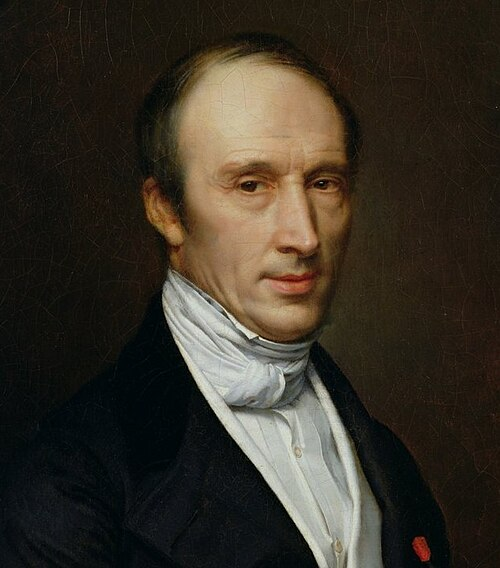
\includegraphics[width=0.82\textwidth]{cauchy.jpg}
    \caption*{(a) \textbf{Augustin-Louis Cauchy (1789--1857)}}
  \end{minipage}
  \hspace{0.08\textwidth}
  \begin{minipage}{0.35\textwidth}
    \centering
    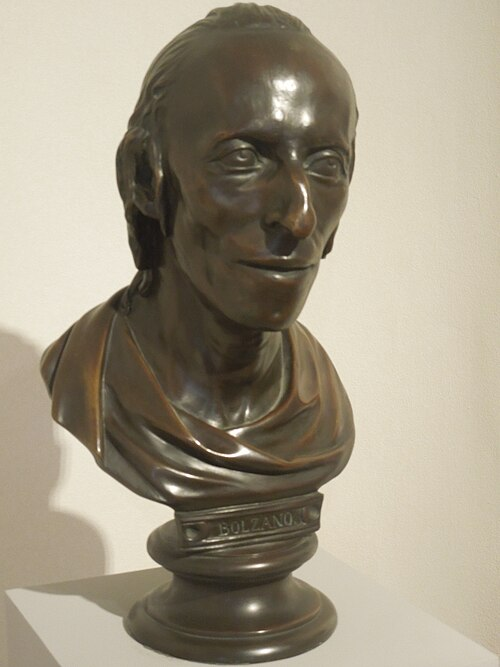
\includegraphics[width=0.82\textwidth]{bolzano.jpg}
    \caption*{(b) \textbf{Bernard Bolzano (1781--1848)}}
  \end{minipage}
  \caption{\textbf{Architects of Modern Rigorous Analysis:} Augustin-Louis Cauchy (who formalized $\varepsilon$-$\delta$ limits, continuity, and Cauchy sequences) and Bernard Bolzano (pioneer of the Bolzano-Weierstrass theorem and intermediate value theorem).}
  \label{fig:cauchy_bolzano}
\end{figure}

\begin{definitionbox}{Convergence of a Sequence ($\varepsilon$-$N$ Formulation)}
A sequence $(u_n)$ is said to \textbf{converge} to a finite real limit $l \in \mathbb{R}$, denoted $\lim_{n \to \infty} u_n = l$ or $u_n \xrightarrow[n \to \infty]{} l$, if:
\begin{equation}
\forall \varepsilon > 0, \quad \exists N_\varepsilon \in \mathbb{N} \quad \text{such that} \quad \forall n \in \mathbb{N}, \quad \left( n > N_\varepsilon \implies |u_n - l| < \varepsilon \right).
\end{equation}
Equivalently: for every interval $(l - \varepsilon, l + \varepsilon)$ centered on $l$, all terms of the sequence from index $N_\varepsilon + 1$ onward lie strictly inside the interval. A sequence that does not converge is called \textbf{divergent}.
\end{definitionbox}

\begin{figure}[htbp]
  \centering
  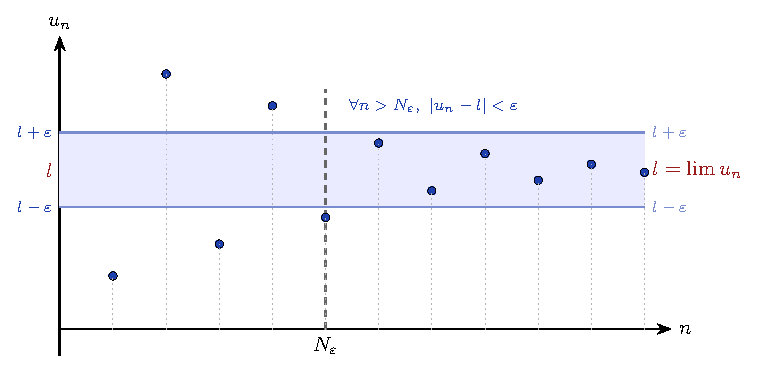
\includegraphics[width=0.90\textwidth]{04_sequence_convergence.pdf}
  \caption{\textbf{Geometric Interpretation of Sequence Convergence:} Given an arbitrary tolerance $\varepsilon > 0$, an index $N_\varepsilon$ exists such that for all indices $n > N_\varepsilon$, all sequence points $u_n$ are permanently trapped within the horizontal $\varepsilon$-tube $(l - \varepsilon, l + \varepsilon)$.}
  \label{fig:seq_convergence}
\end{figure}

\begin{theorembox}{Uniqueness of the Limit and Boundedness}
\begin{enumerate}[leftmargin=1.4em,itemsep=3pt]
  \item \textbf{Uniqueness:} If a sequence $(u_n)$ converges, its limit $l$ is \textbf{unique}:
  \[
  (u_n \to l_1 \quad \text{and} \quad u_n \to l_2) \implies l_1 = l_2.
  \]
  \item \textbf{Boundedness:} Every convergent sequence is \textbf{bounded}:
  \[
  (u_n \to l) \implies \exists M > 0, \quad \forall n \in \mathbb{N}, \quad |u_n| \le M.
  \]
  (\textit{Note:} The converse is false; e.g. $u_n = (-1)^n$ is bounded but divergent).
\end{enumerate}
\end{theorembox}

\begin{definitionbox}{Infinite Limits and Divergence to Infinity}
\begin{enumerate}[leftmargin=1.4em,itemsep=2pt]
  \item $\lim_{n \to \infty} u_n = +\infty \iff \forall A > 0, \ \exists N_A \in \mathbb{N}, \ \forall n > N_A, \ u_n > A$.
  \item $\lim_{n \to \infty} u_n = -\infty \iff \forall B > 0, \ \exists N_B \in \mathbb{N}, \ \forall n > N_B, \ u_n < -B$.
\end{enumerate}
\end{definitionbox}

\section{Fundamental Convergence Criteria}

\begin{theorembox}{The Squeeze (Sandwich / Gendarmes) Theorem}
Let $(u_n), (v_n), (w_n)$ be three real sequences such that:
\begin{enumerate}[leftmargin=1.4em,itemsep=2pt]
  \item There exists an integer $n_0 \in \mathbb{N}$ such that $\forall n \ge n_0, \ v_n \le u_n \le w_n$;
  \item $\lim_{n \to \infty} v_n = \lim_{n \to \infty} w_n = l$.
\end{enumerate}
Then the sequence $(u_n)$ converges and its limit is:
\begin{equation}
\lim_{n \to \infty} u_n = l.
\end{equation}
\end{theorembox}

\begin{theorembox}{The Monotone Convergence Theorem}
\begin{enumerate}[leftmargin=1.4em,itemsep=3pt]
  \item If $(u_n)$ is **monotonically increasing** ($u_{n+1} \ge u_n$) and **bounded above**, then $(u_n)$ converges, and its limit is the supremum of its range:
  \[
  \lim_{n \to \infty} u_n = \sup \{ u_n \mid n \in \mathbb{N} \}.
  \]
  If it is increasing and not bounded above, then $\lim_{n \to \infty} u_n = +\infty$.
  \item If $(u_n)$ is **monotonically decreasing** ($u_{n+1} \le u_n$) and **bounded below**, then $(u_n)$ converges, and its limit is the infimum of its range:
  \[
  \lim_{n \to \infty} u_n = \inf \{ u_n \mid n \in \mathbb{N} \}.
  \]
  If it is decreasing and not bounded below, then $\lim_{n \to \infty} u_n = -\infty$.
\end{enumerate}
\end{theorembox}

\section{Subsequences, Cauchy Sequences, and Adjacent Sequences}

\begin{definitionbox}{Subsequences (Suites Extraites)}
Let $(u_n)_{n \in \mathbb{N}}$ be a sequence. A **subsequence** is a sequence of the form $(u_{\phi(k)})_{k \in \mathbb{N}}$, where:
\[
\phi: \mathbb{N} \longrightarrow \mathbb{N} \quad \text{is a strictly increasing function} \quad (\phi(0) < \phi(1) < \phi(2) < \dots).
\]
Note that for every $k \in \mathbb{N}$, $\phi(k) \ge k$.
If $u_n \to l$, then every subsequence converges to the exact same limit: $u_{\phi(k)} \xrightarrow[k \to \infty]{} l$.
\end{definitionbox}

\begin{theorembox}{The Bolzano-Weierstrass Theorem for Sequences}
Every \textbf{bounded sequence} of real numbers possesses at least one \textbf{convergent subsequence}.
\end{theorembox}

\begin{definitionbox}{Cauchy Sequences and Completeness}
A sequence $(u_n)$ is a \textbf{Cauchy sequence} if its terms become arbitrarily close to each other as their indices grow:
\begin{equation}
\forall \varepsilon > 0, \quad \exists N \in \mathbb{N} \quad \text{such that} \quad \forall p, q \in \mathbb{N}, \quad \left( (p > N \ \land \ q > N) \implies |u_p - u_q| < \varepsilon \right).
\end{equation}
\textbf{The Cauchy Criterion (Completeness of $\mathbb{R}$):}
In the real number field $\mathbb{R}$, a sequence converges to a finite limit if and only if it is a Cauchy sequence:
\[
(u_n) \text{ converges in } \mathbb{R} \iff (u_n) \text{ is a Cauchy sequence}.
\]
\end{definitionbox}

\begin{definitionbox}{Adjacent Sequences (Suites Adjacentes)}
Two sequences $(u_n)$ and $(v_n)$ are said to be \textbf{adjacent} if:
\begin{enumerate}[leftmargin=1.4em,itemsep=2pt]
  \item $(u_n)$ is monotonically increasing;
  \item $(v_n)$ is monotonically decreasing;
  \item $\lim_{n \to \infty} (v_n - u_n) = 0$.
\end{enumerate}
\textbf{Theorem on Adjacent Sequences:}
If $(u_n)$ and $(v_n)$ are adjacent, then:
\begin{itemize}[leftmargin=1.4em,itemsep=1pt]
  \item For all $n \in \mathbb{N}$, $u_n \le v_n$;
  \item Both sequences converge to the **exact same common limit** $l \in \mathbb{R}$:
  \[
  \lim_{n \to \infty} u_n = \lim_{n \to \infty} v_n = l, \qquad \text{and} \quad \forall n \in \mathbb{N}, \quad u_n \le l \le v_n.
  \]
\end{itemize}
\end{definitionbox}

\section{Worked Examples with Step-by-Step Proofs}

\begin{workedexample}{Rigorous Proof of Limit Uniqueness by Contradiction}
Prove from the formal $\varepsilon$-$N$ definition that the limit of a convergent sequence is unique.

\paragraph{Solution and Proof.}
Let $(u_n)$ be a sequence. Assume to the contrary that $(u_n)$ converges to two distinct limits $l_1 \neq l_2$.
Then the distance between them is strictly positive:
\[
|l_1 - l_2| > 0.
\]
Choose $\varepsilon = \frac{|l_1 - l_2|}{2} > 0$.
\begin{enumerate}[leftmargin=1.4em,itemsep=3pt]
  \item Since $u_n \to l_1$, by the definition of limit for this $\varepsilon$, there exists an integer $N_1 \in \mathbb{N}$ such that:
  \[
  \forall n > N_1, \quad |u_n - l_1| < \varepsilon = \frac{|l_1 - l_2|}{2}.
  \]
  \item Since $u_n \to l_2$, there exists an integer $N_2 \in \mathbb{N}$ such that:
  \[
  \forall n > N_2, \quad |u_n - l_2| < \varepsilon = \frac{|l_1 - l_2|}{2}.
  \]
\end{enumerate}
Now choose any index $n_0 > \max(N_1, N_2)$.
For this $n_0$, both inequalities hold simultaneously.
Using the triangle inequality:
\begin{align*}
|l_1 - l_2| &= |(l_1 - u_{n_0}) + (u_{n_0} - l_2)| \\
            &\le |l_1 - u_{n_0}| + |u_{n_0} - l_2| = |u_{n_0} - l_1| + |u_{n_0} - l_2| \\
            &< \frac{|l_1 - l_2|}{2} + \frac{|l_1 - l_2|}{2} = |l_1 - l_2|.
\end{align*}
This yields the strict inequality:
\[
|l_1 - l_2| < |l_1 - l_2|,
\]
which is an undeniable logical contradiction ($x < x$).
Therefore, the assumption that $l_1 \neq l_2$ is false, establishing that:
\[
\mathbf{l_1 = l_2}. \quad \blacksquare
\]
\end{workedexample}

\begin{workedexample}{Verification of Limit via Formal $\varepsilon$-$N$ Argument}
Using the formal $\varepsilon$-$N$ definition of limit, prove that:
\[
\lim_{n \to \infty} \frac{3n + 5}{2n - 1} = \frac{3}{2}.
\]

\paragraph{Solution and Proof.}
Let $\varepsilon > 0$ be given. We must find an integer $N_\varepsilon \in \mathbb{N}$ such that for all $n > N_\varepsilon$:
\[
\left| \frac{3n + 5}{2n - 1} - \frac{3}{2} \right| < \varepsilon.
\]
Compute the algebraic difference over a common denominator:
\[
\frac{3n + 5}{2n - 1} - \frac{3}{2} = \frac{2(3n + 5) - 3(2n - 1)}{2(2n - 1)} = \frac{(6n + 10) - (6n - 3)}{2(2n - 1)} = \frac{13}{2(2n - 1)}.
\]
For $n \ge 1$, $2n - 1 > 0$, so the absolute value can be removed:
\[
\left| \frac{3n + 5}{2n - 1} - \frac{3}{2} \right| = \frac{13}{4n - 2}.
\]
We require:
\[
\frac{13}{4n - 2} < \varepsilon \iff 4n - 2 > \frac{13}{\varepsilon} \iff 4n > \frac{13}{\varepsilon} + 2 \iff n > \frac{13}{4\varepsilon} + \frac{1}{2}.
\]
By the Archimedean property of $\mathbb{R}$, we can choose:
\[
N_\varepsilon = \left\lfloor \frac{13}{4\varepsilon} + \frac{1}{2} \right\rfloor + 1 \in \mathbb{N}.
\]
Then for any $n > N_\varepsilon$:
\[
n > \frac{13}{4\varepsilon} + \frac{1}{2} \implies 4n - 2 > \frac{13}{\varepsilon} \implies \left| \frac{3n + 5}{2n - 1} - \frac{3}{2} \right| = \frac{13}{4n - 2} < \varepsilon.
\]
This completes the formal proof that $\mathbf{\lim_{n \to \infty} \frac{3n + 5}{2n - 1} = \frac{3}{2}}$. $\blacksquare$
\end{workedexample}

\begin{workedexample}{Convergence of a Recurring Sequence via Monotone Convergence}
Consider the sequence $(u_n)_{n \in \mathbb{N}}$ defined by recurrence:
\[
u_0 = 1, \qquad u_{n+1} = \sqrt{2 + u_n} \quad \text{for all } n \ge 0.
\]
\begin{enumerate}[leftmargin=1.4em,itemsep=2pt]
  \item Prove by mathematical induction that for all $n \in \mathbb{N}$, $1 \le u_n < 2$.
  \item Prove by mathematical induction that $(u_n)$ is strictly increasing.
  \item Deduce that $(u_n)$ converges and calculate its limit $l$.
\end{enumerate}

\paragraph{Solution and Proof.}
\textbf{1. Boundedness by Induction ($1 \le u_n < 2$):}
\begin{itemize}[leftmargin=1.4em,itemsep=2pt]
  \item \textbf{Base step ($n = 0$):} $u_0 = 1$, which satisfies $1 \le 1 < 2$. True.
  \item \textbf{Inductive step:} Assume $1 \le u_k < 2$ for some $k \ge 0$.
  Adding $2$: $3 \le 2 + u_k < 4$.
  Since the square root function is strictly increasing on $\mathbb{R}^+$:
  \[
  \sqrt{3} \le \sqrt{2 + u_k} < \sqrt{4} = 2.
  \]
  Since $1 < \sqrt{3} \approx 1.732$, we have $1 \le u_{k+1} < 2$.
\end{itemize}
Thus, by induction, $1 \le u_n < 2$ for all $n \in \mathbb{N}$.

\textbf{2. Monotonicity by Induction ($u_{n+1} > u_n$):}
\begin{itemize}[leftmargin=1.4em,itemsep=2pt]
  \item \textbf{Base step ($n = 0$):} $u_0 = 1$ and $u_1 = \sqrt{2 + 1} = \sqrt{3} \approx 1.732 > 1 = u_0$. True.
  \item \textbf{Inductive step:} Assume $u_{k+1} > u_k$ for some $k \ge 0$.
  Adding $2$: $2 + u_{k+1} > 2 + u_k$.
  Taking square roots:
  \[
  \sqrt{2 + u_{k+1}} > \sqrt{2 + u_k} \implies u_{k+2} > u_{k+1}.
  \]
\end{itemize}
Thus, $(u_n)$ is strictly increasing.

\textbf{3. Convergence and Limit Calculation:}
Because $(u_n)$ is strictly increasing and bounded above by $2$, the **Monotone Convergence Theorem** guarantees that $(u_n)$ converges to a finite limit $l \in [1, 2]$:
\[
\lim_{n \to \infty} u_n = l.
\]
Since the function $f(x) = \sqrt{2 + x}$ is continuous on $[1, 2]$:
\[
\lim_{n \to \infty} u_{n+1} = f\left( \lim_{n \to \infty} u_n \right) \implies l = \sqrt{2 + l}.
\]
Squaring both sides ($l \ge 1 > 0$):
\[
l^2 = 2 + l \implies l^2 - l - 2 = 0 \implies (l - 2)(l + 1) = 0.
\]
The roots are $l = 2$ and $l = -1$.
Since $u_n \ge 1$ for all $n$, the limit must be positive ($l \ge 1$), which rejects $l = -1$.
Therefore:
\[
\mathbf{\lim_{n \to \infty} u_n = 2}. \quad \blacksquare
\]
\end{workedexample}

\begin{workedexample}{Euler's Constant $e$ via Adjacent Sequences}
Define the two sequences for $n \ge 1$:
\[
u_n = \left( 1 + \frac{1}{n} \right)^n, \qquad v_n = \left( 1 + \frac{1}{n} \right)^{n+1}.
\]
\begin{enumerate}[leftmargin=1.4em,itemsep=2pt]
  \item Show that $v_n = u_n \left( 1 + \frac{1}{n} \right)$ and that $\lim_{n \to \infty} (v_n - u_n) = 0$.
  \item Given that $(u_n)$ is strictly increasing and $(v_n)$ is strictly decreasing, prove that $(u_n)$ and $(v_n)$ are adjacent.
  \item Conclude on the existence of Euler's number $e = \lim_{n \to \infty} \left( 1 + \frac{1}{n} \right)^n$ and establish the framing $u_n < e < v_n$.
\end{enumerate}

\paragraph{Solution and Proof.}
\textbf{1. Ratio and Difference:}
\[
v_n = \left( 1 + \frac{1}{n} \right)^{n+1} = \left( 1 + \frac{1}{n} \right)^n \cdot \left( 1 + \frac{1}{n} \right) = u_n \left( 1 + \frac{1}{n} \right).
\]
The difference is:
\[
v_n - u_n = u_n \left( 1 + \frac{1}{n} \right) - u_n = \frac{u_n}{n}.
\]
By the binomial theorem, $u_n = \sum_{k=0}^n \binom{n}{k} \frac{1}{n^k} = 1 + 1 + \frac{1}{2!} \left(1 - \frac{1}{n}\right) + \dots < \sum_{k=0}^\infty \frac{1}{k!} = 3$.
Since $0 < u_n < 3$:
\[
0 < v_n - u_n = \frac{u_n}{n} < \frac{3}{n}.
\]
Taking limits as $n \to \infty$, since $\lim \frac{3}{n} = 0$, by the squeeze theorem:
\[
\lim_{n \to \infty} (v_n - u_n) = 0.
\]

\textbf{2. Adjacency of the Sequences:}
\begin{itemize}[leftmargin=1.4em,itemsep=1pt]
  \item $(u_n)$ is strictly increasing;
  \item $(v_n)$ is strictly decreasing;
  \item $\lim_{n \to \infty} (v_n - u_n) = 0$.
\end{itemize}
All three conditions of the **Adjacent Sequences Theorem** are satisfied.

\textbf{3. Existence and Definition of $e$:}
By the theorem on adjacent sequences, $(u_n)$ and $(v_n)$ converge to a unique common limit, which defines **Euler's number** $e$:
\[
\mathbf{\lim_{n \to \infty} \left( 1 + \frac{1}{n} \right)^n = \lim_{n \to \infty} \left( 1 + \frac{1}{n} \right)^{n+1} = e \approx 2.718\,281\,828\dots}
\]
Furthermore, for every positive integer $n \ge 1$:
\[
\mathbf{\left( 1 + \frac{1}{n} \right)^n < e < \left( 1 + \frac{1}{n} \right)^{n+1}}. \quad \blacksquare
\]
\end{workedexample}

\chapter{Real Functions of a Real Variable: Limits, Continuity \& Derivatives}
\label{chap:functions_derivatives}

\section{Limits of Real Functions and the $\varepsilon$-$\delta$ Definition}

Let $I \subseteq \mathbb{R}$ be an interval and $f: I \longrightarrow \mathbb{R}$ a real function. Let $x_0 \in \mathbb{R}$ be an accumulation point of $I$.

\begin{figure}[htbp]
  \centering
  \begin{minipage}{0.30\textwidth}
    \centering
    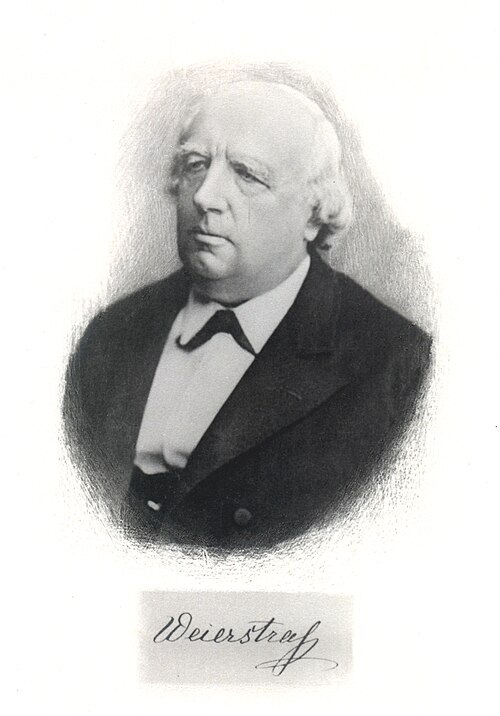
\includegraphics[width=0.88\textwidth]{weierstrass.jpg}
    \caption*{(a) \textbf{Karl Weierstrass (1815--1897)}}
  \end{minipage}
  \hfill
  \begin{minipage}{0.30\textwidth}
    \centering
    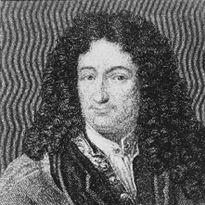
\includegraphics[width=0.88\textwidth]{rolle.jpg}
    \caption*{(b) \textbf{Michel Rolle (1652--1719)}}
  \end{minipage}
  \hfill
  \begin{minipage}{0.30\textwidth}
    \centering
    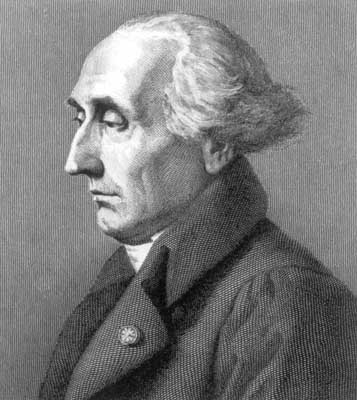
\includegraphics[width=0.88\textwidth]{lagrange.jpg}
    \caption*{(c) \textbf{Joseph-Louis Lagrange (1736--1813)}}
  \end{minipage}
  \caption{\textbf{Masters of Differential Calculus:} Karl Weierstrass ("Father of Modern Analysis", creator of the static $\varepsilon$-$\delta$ definition), Michel Rolle (formulator of Rolle's Theorem in 1691), and Joseph-Louis Lagrange (discoverer of the Mean Value Theorem and remainder formulas for Taylor series).}
  \label{fig:analysis_masters}
\end{figure}

\begin{definitionbox}{Formal $\varepsilon$-$\delta$ Definition of Functional Limit}
The function $f$ has a \textbf{limit} $L \in \mathbb{R}$ as $x$ approaches $x_0$, written $\lim_{x \to x_0} f(x) = L$, if:
\begin{equation}
\forall \varepsilon > 0, \quad \exists \delta > 0 \quad \text{such that} \quad \forall x \in I, \quad \left( 0 < |x - x_0| < \delta \implies |f(x) - L| < \varepsilon \right).
\end{equation}
\end{definitionbox}

\begin{figure}[htbp]
  \centering
  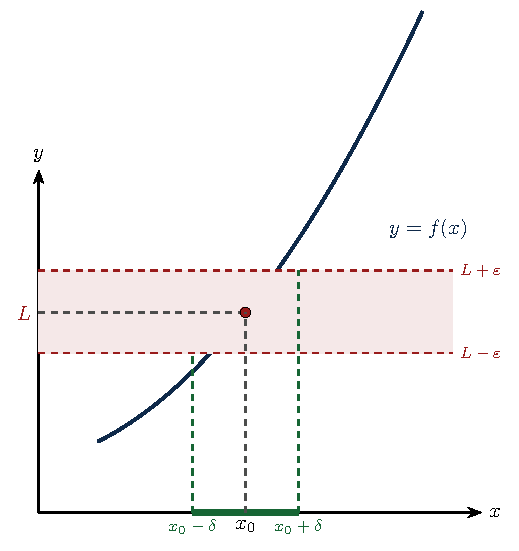
\includegraphics[width=0.88\textwidth]{05_epsilon_delta_limit.pdf}
  \caption{\textbf{Weierstrass $\varepsilon$-$\delta$ Neighborhood Geometry:} For any target band $(L - \varepsilon, L + \varepsilon)$ along the $y$-axis, there exists a surrounding interval $(x_0 - \delta, x_0 + \delta)$ on the $x$-axis whose functional images fall strictly within the band.}
  \label{fig:eps_delta}
\end{figure}

\begin{theorembox}{Sequential Characterization of Functional Limits (Heine's Theorem)}
Let $f: I \longrightarrow \mathbb{R}$ and $x_0$ an accumulation point of $I$. The following assertions are logically equivalent:
\begin{enumerate}[leftmargin=1.4em,itemsep=2pt]
  \item $\lim_{x \to x_0} f(x) = L$;
  \item For every sequence $(x_n)_{n \in \mathbb{N}}$ in $I \setminus \{x_0\}$ converging to $x_0$, the image sequence $(f(x_n))$ converges to $L$:
  \[
  \forall (x_n) \subset I \setminus \{x_0\}, \quad \left( \lim_{n \to \infty} x_n = x_0 \implies \lim_{n \to \infty} f(x_n) = L \right).
  \]
\end{enumerate}
\textit{Corollary (Disproof Criterion):} If two sequences $x_n \to x_0$ and $x'_n \to x_0$ yield different limits $\lim f(x_n) \neq \lim f(x'_n)$, then $\lim_{x \to x_0} f(x)$ does not exist (e.g. $f(x) = \sin(1/x)$ as $x \to 0$).
\end{theorembox}

\section{Continuity of Real Functions}

\begin{definitionbox}{Continuity at a Point and on an Interval}
\begin{enumerate}[leftmargin=1.4em,itemsep=3pt]
  \item A function $f: I \longrightarrow \mathbb{R}$ is \textbf{continuous at a point} $x_0 \in I$ if:
  \[
  \lim_{x \to x_0} f(x) = f(x_0) \iff \forall \varepsilon > 0, \ \exists \delta > 0, \ \forall x \in I, \ (|x - x_0| < \delta \implies |f(x) - f(x_0)| < \varepsilon).
  \]
  \item $f$ is \textbf{continuous on the interval} $I$ if it is continuous at every point $x_0 \in I$. We write $f \in \mathcal{C}^0(I)$ or $f \in \mathcal{C}(I, \mathbb{R})$.
\end{enumerate}
\end{definitionbox}

\begin{theorembox}{The Intermediate Value Theorem (Théorème des Valeurs Intermédiaires)}
Let $f: [a, b] \longrightarrow \mathbb{R}$ be a continuous function on a closed bounded interval $[a, b]$.
\begin{enumerate}[leftmargin=1.4em,itemsep=2pt]
  \item For every real number $y$ lying between $f(a)$ and $f(b)$, there exists at least one real number $c \in [a, b]$ such that:
  \[
  f(c) = y.
  \]
  \item \textbf{Bolzano's Root Theorem:} If $f(a) \cdot f(b) < 0$ (opposite signs at endpoints), then there exists at least one root $c \in (a, b)$ such that $f(c) = 0$.
\end{enumerate}
\end{theorembox}

\begin{theorembox}{The Extreme Value Theorem (Weierstrass's Theorem)}
Let $f: [a, b] \longrightarrow \mathbb{R}$ be a continuous function on a compact (closed and bounded) interval $[a, b]$.
Then $f$ is \textbf{bounded} and \textbf{attains its bounds}:
\begin{equation}
\exists x_{\min}, x_{\max} \in [a, b] \quad \text{such that} \quad f(x_{\min}) = \inf_{x \in [a, b]} f(x) \quad \text{and} \quad f(x_{\max}) = \sup_{x \in [a, b]} f(x).
\end{equation}
Thus, $f([a, b]) = [m, M]$ is itself a closed and bounded interval.
\end{theorembox}

\section{Differential Calculus: Definitions and Core Properties}

\begin{definitionbox}{The Derivative at a Point}
Let $f: I \longrightarrow \mathbb{R}$ and $x_0$ an interior point of $I$.
The function $f$ is \textbf{differentiable at $x_0$} if the difference quotient has a finite limit as $h \to 0$:
\begin{equation}
f'(x_0) = \lim_{h \to 0} \frac{f(x_0 + h) - f(x_0)}{h} = \lim_{x \to x_0} \frac{f(x) - f(x_0)}{x - x_0}.
\end{equation}
$f'(x_0)$ is the \textbf{derivative} of $f$ at $x_0$.
Geometrically, $f'(x_0)$ is the exact slope of the tangent line to the curve $y = f(x)$ at $(x_0, f(x_0))$:
\[
y = f(x_0) + f'(x_0)(x - x_0).
\]
\end{definitionbox}

\begin{theorembox}{Differentiability Implies Continuity}
If $f$ is differentiable at $x_0$, then $f$ is necessarily continuous at $x_0$:
\begin{equation}
f \text{ differentiable at } x_0 \implies f \text{ continuous at } x_0.
\end{equation}
(\textit{Caution:} The converse is false! The absolute value function $f(x) = |x|$ is continuous at $x = 0$ but not differentiable at $x = 0$).
\end{theorembox}

\begin{propbox}{Algebra of Derivatives}
Let $u, v: I \longrightarrow \mathbb{R}$ be differentiable at $x$:
\begin{enumerate}[leftmargin=1.4em,itemsep=2pt]
  \item \textbf{Linearity:} $(\alpha u + \beta v)'(x) = \alpha u'(x) + \beta v'(x)$ for all $\alpha, \beta \in \mathbb{R}$.
  \item \textbf{Leibniz Product Rule:} $(u \cdot v)'(x) = u'(x) v(x) + u(x) v'(x)$.
  \item \textbf{Quotient Rule:} $\left( \frac{u}{v} \right)'(x) = \frac{u'(x) v(x) - u(x) v'(x)}{[v(x)]^2}$ (provided $v(x) \neq 0$).
  \item \textbf{Chain Rule:} If $f$ is differentiable at $x$ and $g$ is differentiable at $f(x)$:
  \[
  (g \circ f)'(x) = g'(f(x)) \cdot f'(x).
  \]
  \item \textbf{Derivative of Inverse Function:} If $f$ is a bijective differentiable function with $f'(x_0) \neq 0$:
  \[
  (f^{-1})'(y_0) = \frac{1}{f'(x_0)} = \frac{1}{f'(f^{-1}(y_0))} \quad \text{where } y_0 = f(x_0).
  \]
\end{enumerate}
\end{propbox}

\section{Fundamental Theorems of Differential Calculus}

\begin{theorembox}{Fermat's Theorem on Local Extrema}
Let $f: (a, b) \longrightarrow \mathbb{R}$ be differentiable on the open interval $(a, b)$.
If $f$ attains a **local extremum** (local maximum or local minimum) at an interior point $c \in (a, b)$, then:
\begin{equation}
f'(c) = 0.
\end{equation}
Points where $f'(c) = 0$ are called \textbf{critical points} (or stationary points).
\end{theorembox}

\begin{figure}[htbp]
  \centering
  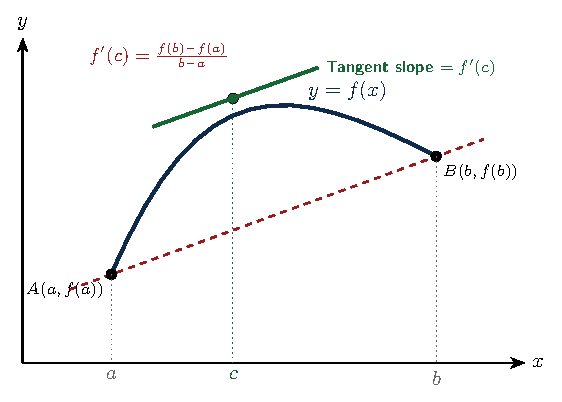
\includegraphics[width=0.88\textwidth]{06_rolle_mvt.pdf}
  \caption{\textbf{Rolle's and Mean Value Theorem Geometry:} The secant chord connecting endpoint coordinates $(a, f(a))$ and $(b, f(b))$ has slope $\frac{f(b) - f(a)}{b - a}$. There exists at least one interior point $c \in (a, b)$ where the tangent line to the curve is strictly parallel to the secant line ($f'(c) = \text{slope}$).}
  \label{fig:rolle_mvt}
\end{figure}

\begin{theorembox}{Rolle's Theorem (1691)}
Let $f: [a, b] \longrightarrow \mathbb{R}$ be a function satisfying:
\begin{enumerate}[leftmargin=1.4em,itemsep=2pt]
  \item $f$ is continuous on the closed interval $[a, b]$;
  \item $f$ is differentiable on the open interval $(a, b)$;
  \item $f(a) = f(b)$.
\end{enumerate}
Then there exists at least one interior point $c \in (a, b)$ such that:
\begin{equation}
f'(c) = 0.
\end{equation}
\end{theorembox}

\begin{theorembox}{The Mean Value Theorem (Théorème des Accroissements Finis / TAF)}
Let $f: [a, b] \longrightarrow \mathbb{R}$ be continuous on $[a, b]$ and differentiable on $(a, b)$.
Then there exists at least one point $c \in (a, b)$ such that:
\begin{equation}
f(b) - f(a) = f'(c) \cdot (b - a) \iff f'(c) = \frac{f(b) - f(a)}{b - a}.
\end{equation}
\end{theorembox}

\begin{propbox}{Corollaries of the Mean Value Theorem}
Let $f$ be differentiable on an interval $I$:
\begin{enumerate}[leftmargin=1.4em,itemsep=2pt]
  \item \textbf{Constant Function Criterion:} $\forall x \in I, f'(x) = 0 \iff f$ is constant on $I$.
  \item \textbf{Monotonicity Criteria:}
  \begin{itemize}[leftmargin=1.2em,itemsep=1pt]
    \item $f'(x) \ge 0$ on $I \iff f$ is monotonically increasing on $I$.
    \item $f'(x) \le 0$ on $I \iff f$ is monotonically decreasing on $I$.
    \item $f'(x) > 0$ on $I \implies f$ is strictly increasing on $I$.
  \end{itemize}
  \item \textbf{Mean Value Inequality (Inégalité des Accroissements Finis):}
  If $|f'(x)| \le M$ for all $x \in I$, then for all $x, y \in I$:
  \[
  |f(x) - f(y)| \le M |x - y|.
  \]
  (The function is Lipschitz continuous with Lipschitz constant $M$).
\end{enumerate}
\end{propbox}

\begin{theorembox}{Cauchy's Generalized Mean Value Theorem and L'Hôpital's Rule}
\begin{enumerate}[leftmargin=1.4em,itemsep=3pt]
  \item \textbf{Cauchy's Extended Mean Value Theorem:}
  If $f, g: [a, b] \longrightarrow \mathbb{R}$ are continuous on $[a, b]$ and differentiable on $(a, b)$, and $g'(x) \neq 0$ on $(a, b)$, then there exists $c \in (a, b)$ such that:
  \[
  \frac{f(b) - f(a)}{g(b) - g(a)} = \frac{f'(c)}{g'(c)}.
  \]
  \item \textbf{L'Hôpital's Rule:} If $\lim_{x \to x_0} f(x) = \lim_{x \to x_0} g(x) = 0$ (or $\pm\infty$), and $\lim_{x \to x_0} \frac{f'(x)}{g'(x)} = L \in \mathbb{R} \cup \{\pm\infty\}$, then:
  \[
  \lim_{x \to x_0} \frac{f(x)}{g(x)} = \lim_{x \to x_0} \frac{f'(x)}{g'(x)} = L.
  \]
\end{enumerate}
\end{theorembox}

\section{Worked Examples with Step-by-Step Proofs}

\begin{workedexample}{Rigorous Proof of Rolle's Theorem from Weierstrass's Theorem}
Provide the complete, rigorous analytical proof of Rolle's Theorem using the Extreme Value Theorem and Fermat's Theorem.

\paragraph{Solution and Proof.}
Let $f: [a, b] \longrightarrow \mathbb{R}$ satisfy the three hypotheses of Rolle's Theorem:
(1) $f$ is continuous on $[a, b]$, (2) $f$ is differentiable on $(a, b)$, and (3) $f(a) = f(b)$.

By the **Weierstrass Extreme Value Theorem**, because $f$ is continuous on the compact interval $[a, b]$, it is bounded and attains both its absolute minimum $m$ and absolute maximum $M$ at points $x_{\min}, x_{\max} \in [a, b]$:
\[
m = f(x_{\min}) = \min_{x \in [a, b]} f(x), \qquad M = f(x_{\max}) = \max_{x \in [a, b]} f(x).
\]
We now examine two mutually exclusive and exhaustive cases:
\begin{itemize}[leftmargin=1.4em,itemsep=3pt]
  \item \textbf{Case 1: $m = M$ (Constant Function).}
  If the minimum equals the maximum, then for all $x \in [a, b]$, $m \le f(x) \le M \implies f(x) = m$.
  Thus $f$ is a constant function on $[a, b]$.
  Its derivative is identically zero everywhere on $(a, b)$:
  \[
  \forall x \in (a, b), \quad f'(x) = 0.
  \]
  Any point $c \in (a, b)$ satisfies $f'(c) = 0$.

  \item \textbf{Case 2: $m < M$ (Non-constant Function).}
  Since $f(a) = f(b)$, it is impossible for both extrema to occur simultaneously at the boundary endpoints $\{a, b\}$.
  Indeed, if both occurred at the endpoints, we would have $m = f(a) = f(b) = M$, which contradicts $m < M$.
  Therefore, at least one of the two extrema must occur at an **interior point** $c \in (a, b)$:
  \begin{itemize}[leftmargin=1.2em,itemsep=1pt]
    \item Either $x_{\max} \in (a, b)$, in which case we set $c = x_{\max}$;
    \item Or $x_{\min} \in (a, b)$, in which case we set $c = x_{\min}$.
  \end{itemize}
  Since $c \in (a, b)$, $f$ has a local extremum at the interior point $c$.
  Moreover, by hypothesis (2), $f$ is differentiable at $c$.
  By **Fermat's Theorem on Local Extrema**, the derivative at an interior extremum must vanish:
  \[
  f'(c) = 0.
  \]
\end{itemize}
In both cases, we have established the existence of at least one point $c \in (a, b)$ such that $\mathbf{f'(c) = 0}$. $\blacksquare$
\end{workedexample}

\begin{workedexample}{Rigorous Proof of the Mean Value Theorem from Rolle's Theorem}
Derive the Mean Value Theorem by constructing an auxiliary function that satisfies Rolle's Theorem.

\paragraph{Solution and Proof.}
Let $f: [a, b] \longrightarrow \mathbb{R}$ be continuous on $[a, b]$ and differentiable on $(a, b)$.
The secant line connecting $(a, f(a))$ and $(b, f(b))$ has equation:
\[
y = f(a) + \frac{f(b) - f(a)}{b - a}(x - a).
\]
Consider the auxiliary function $\phi: [a, b] \longrightarrow \mathbb{R}$ measuring the vertical deviation between the curve $y = f(x)$ and the secant line:
\[
\phi(x) = f(x) - \left[ f(a) + \frac{f(b) - f(a)}{b - a}(x - a) \right].
\]
Let us verify the three hypotheses of Rolle's Theorem for $\phi$:
\begin{enumerate}[leftmargin=1.4em,itemsep=2pt]
  \item \textbf{Continuity on $[a, b]$:} $\phi$ is the difference of $f$ (continuous on $[a, b]$) and an affine linear function (continuous on $\mathbb{R}$). Hence $\phi$ is continuous on $[a, b]$.
  \item \textbf{Differentiability on $(a, b)$:} $\phi$ is differentiable on $(a, b)$ as the difference of differentiable functions, with derivative:
  \[
  \phi'(x) = f'(x) - \frac{f(b) - f(a)}{b - a}.
  \]
  \item \textbf{Equal Endpoint Values:}
  \[
  \phi(a) = f(a) - \left[ f(a) + \frac{f(b) - f(a)}{b - a}(a - a) \right] = f(a) - f(a) = 0.
  \]
  \[
  \phi(b) = f(b) - \left[ f(a) + \frac{f(b) - f(a)}{b - a}(b - a) \right] = f(b) - [f(a) + f(b) - f(a)] = 0.
  \]
  Thus $\phi(a) = \phi(b) = 0$.
\end{enumerate}
All three conditions of Rolle's Theorem are satisfied by $\phi$.
Therefore, there exists at least one point $c \in (a, b)$ such that:
\[
\phi'(c) = 0 \implies f'(c) - \frac{f(b) - f(a)}{b - a} = 0 \implies \mathbf{f'(c) = \frac{f(b) - f(a)}{b - a}}. \quad \blacksquare
\]
\end{workedexample}

\begin{workedexample}{Proving Classical Inequalities via the Mean Value Theorem}
Using the Mean Value Theorem:
\begin{enumerate}[leftmargin=1.4em,itemsep=2pt]
  \item Prove that for all real numbers $x > 0$:
  \[
  \frac{x}{1 + x} < \ln(1 + x) < x.
  \]
  \item Prove that for all $x \in \mathbb{R}$, $|\sin x| \le |x|$.
\end{enumerate}

\paragraph{Solution and Proof.}
\textbf{1. Logarithmic Inequality:}
Fix $x > 0$ and consider the function $f(t) = \ln(1 + t)$ on the interval $[0, x]$.
\begin{itemize}[leftmargin=1.4em,itemsep=2pt]
  \item $f$ is continuous on $[0, x]$ and differentiable on $(0, x)$, with derivative $f'(t) = \frac{1}{1 + t}$.
  \item By the Mean Value Theorem, there exists $c \in (0, x)$ such that:
  \[
  \frac{f(x) - f(0)}{x - 0} = f'(c) \implies \frac{\ln(1 + x) - \ln(1)}{x} = \frac{1}{1 + c} \implies \ln(1 + x) = \frac{x}{1 + c}.
  \]
  \item Since $0 < c < x$, we have $1 < 1 + c < 1 + x$.
  Inverting the inequalities:
  \[
  \frac{1}{1 + x} < \frac{1}{1 + c} < 1.
  \]
  Multiplying through by $x > 0$:
  \[
  \mathbf{\frac{x}{1 + x} < \ln(1 + x) < x}.
  \]
\end{itemize}

\textbf{2. Sine Inequality:}
Consider $g(t) = \sin t$.
For $x = 0$, $|\sin 0| = 0 \le 0$ holds trivially.
For $x \neq 0$, apply the Mean Value Theorem on the interval between $0$ and $x$:
\[
\frac{\sin x - \sin 0}{x - 0} = \cos(c) \quad \text{for some } c \text{ between } 0 \text{ and } x.
\]
Taking absolute values:
\[
\frac{|\sin x|}{|x|} = |\cos c|.
\]
Since $|\cos c| \le 1$ for all real $c$:
\[
\frac{|\sin x|}{|x|} \le 1 \implies \mathbf{|\sin x| \le |x|}. \quad \blacksquare
\]
\end{workedexample}

\begin{workedexample}{Bijective Inverse Function Derivative}
Consider the function $f: \mathbb{R} \longrightarrow \mathbb{R}$ defined by:
\[
f(x) = x^3 + 2x - 1.
\]
\begin{enumerate}[leftmargin=1.4em,itemsep=2pt]
  \item Prove that $f$ is a bijection from $\mathbb{R}$ onto $\mathbb{R}$.
  \item Calculate $f(1)$.
  \item Compute the derivative of the inverse function at $y_0 = 2$, namely $(f^{-1})'(2)$.
\end{enumerate}

\paragraph{Solution and Proof.}
\textbf{1. Proof of Bijectivity:}
$f$ is a polynomial, hence continuous and infinitely differentiable on $\mathbb{R}$.
Its derivative is:
\[
f'(x) = 3x^2 + 2.
\]
For all $x \in \mathbb{R}$, $3x^2 \ge 0 \implies f'(x) \ge 2 > 0$.
Since $f'(x) > 0$ everywhere, $f$ is **strictly increasing** on $\mathbb{R}$.
Furthermore, examining limits at infinity:
\[
\lim_{x \to -\infty} f(x) = -\infty, \qquad \lim_{x \to +\infty} f(x) = +\infty.
\]
By the **Continuous Bijection Theorem**, a strictly increasing continuous function on $\mathbb{R}$ is a bijection from $\mathbb{R}$ onto $\mathbb{R}$.

\textbf{2. Evaluation at $x = 1$:}
\[
f(1) = 1^3 + 2(1) - 1 = 1 + 2 - 1 = \mathbf{2}.
\]

\textbf{3. Derivative of the Inverse Function at $y_0 = 2$:}
Since $f(1) = 2$, we have $f^{-1}(2) = 1$.
Using the formula for the derivative of the inverse function:
\[
(f^{-1})'(2) = \frac{1}{f'(f^{-1}(2))} = \frac{1}{f'(1)}.
\]
Compute $f'(1)$:
\[
f'(1) = 3(1)^2 + 2 = 3 + 2 = 5 \neq 0.
\]
Therefore:
\[
\mathbf{(f^{-1})'(2) = \frac{1}{5} = 0.2}. \quad \blacksquare
\]
\end{workedexample}

\chapter{Taylor Expansions, Asymptotic Developments \& Riemann Integration}
\label{chap:taylor_integrals}

\section{Higher-Order Derivatives and Leibniz's Formula}

Let $f: I \longrightarrow \mathbb{R}$ be an $n$-times differentiable function on an interval $I$. The successive derivatives are defined recursively by $f^{(0)} = f$, $f^{(1)} = f'$, and $f^{(k+1)} = (f^{(k)})'$. If $f^{(n)}$ is continuous on $I$, we write $f \in \mathcal{C}^n(I)$. If $f$ is infinitely differentiable, $f \in \mathcal{C}^\infty(I)$.

\begin{figure}[htbp]
  \centering
  \begin{minipage}{0.30\textwidth}
    \centering
    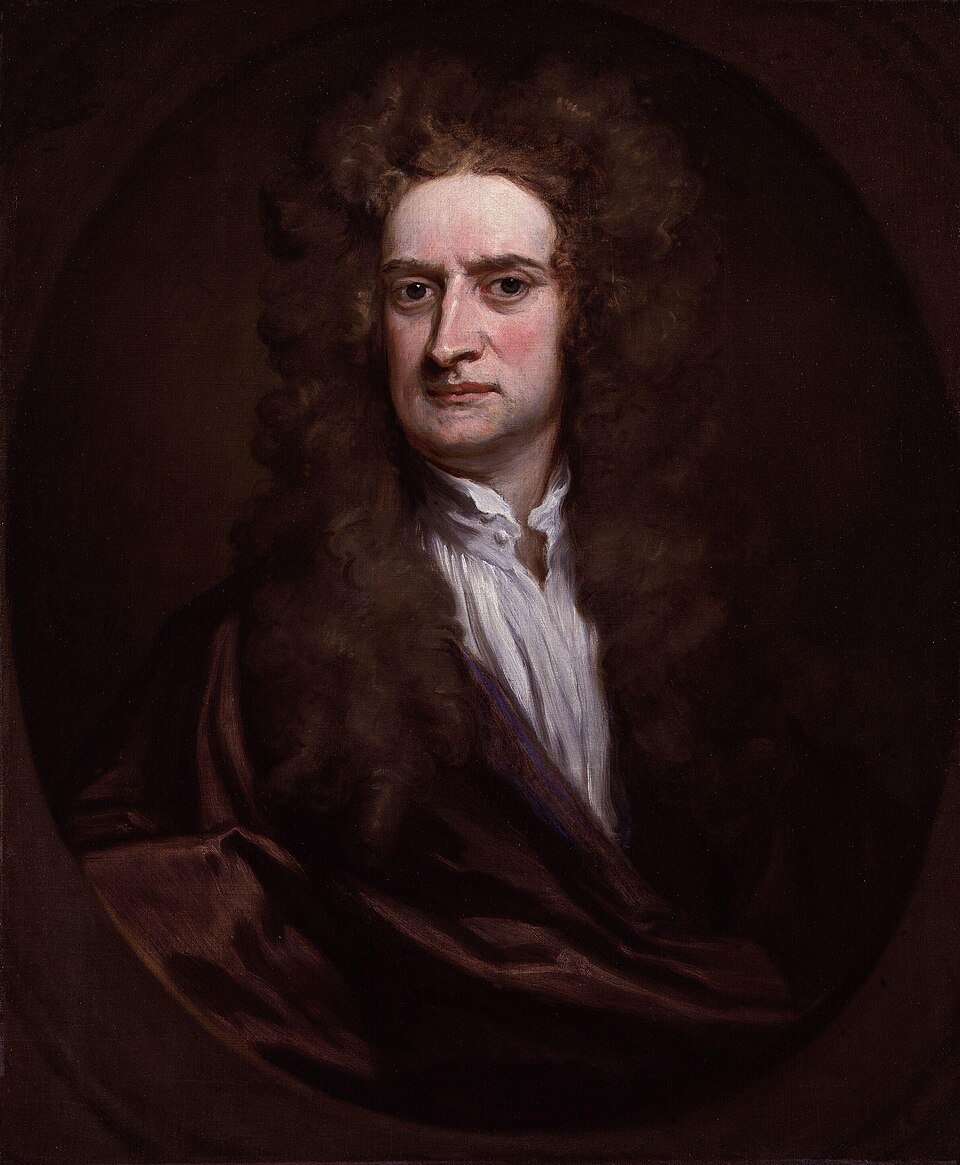
\includegraphics[width=0.88\textwidth]{newton.jpg}
    \caption*{(a) \textbf{Isaac Newton (1642--1727)}}
  \end{minipage}
  \hfill
  \begin{minipage}{0.30\textwidth}
    \centering
    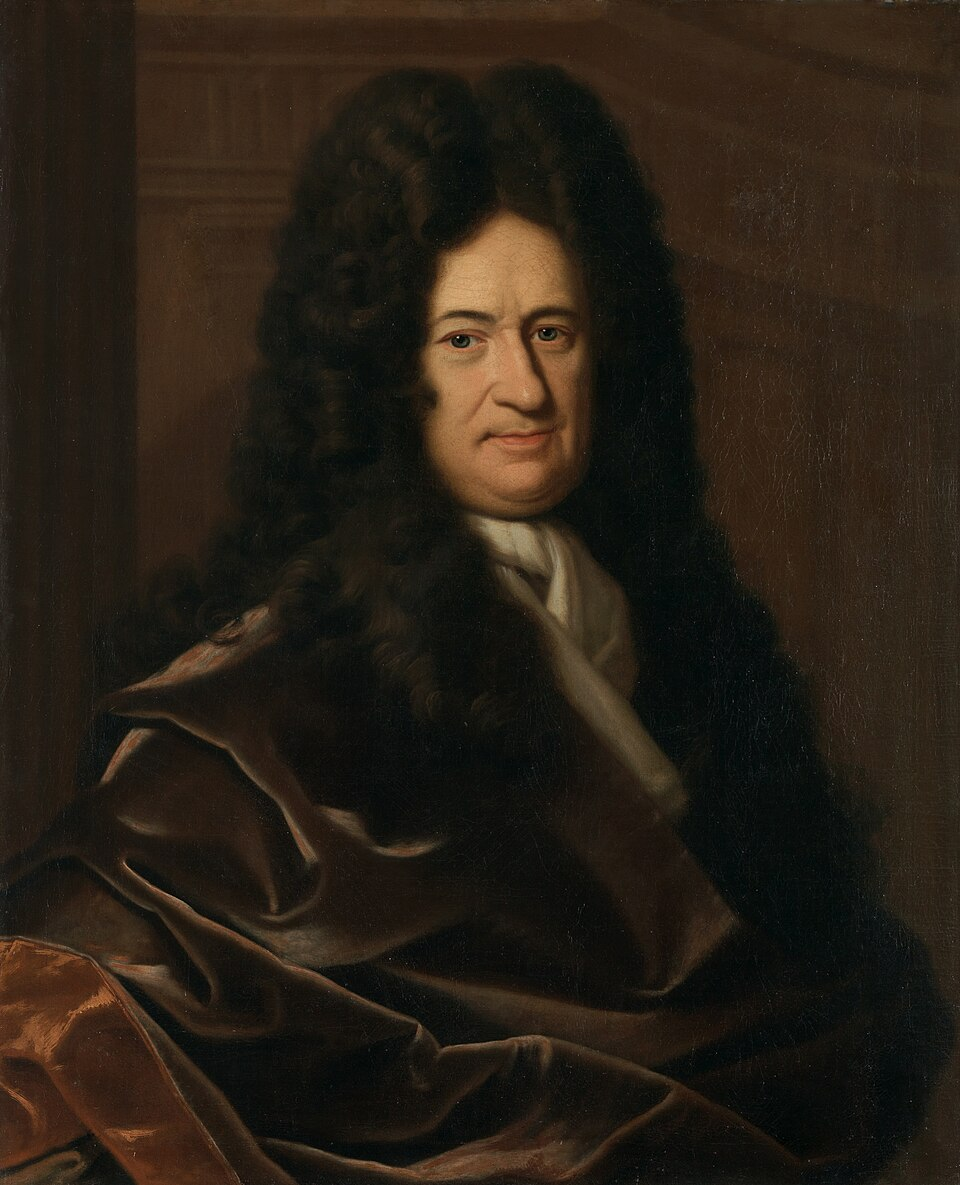
\includegraphics[width=0.88\textwidth]{leibniz.jpg}
    \caption*{(b) \textbf{Gottfried Leibniz (1646--1716)}}
  \end{minipage}
  \hfill
  \begin{minipage}{0.30\textwidth}
    \centering
    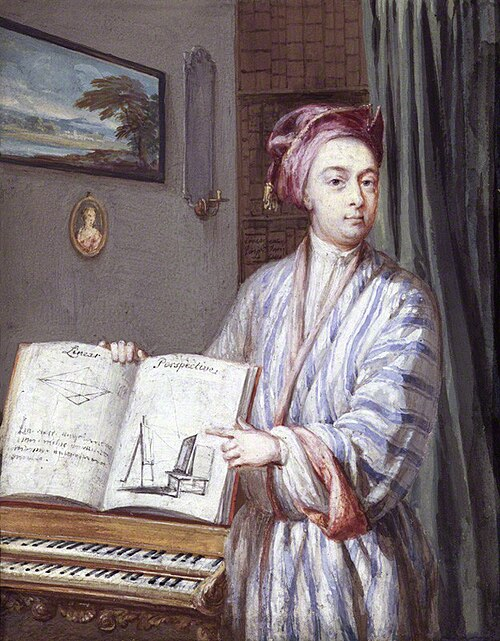
\includegraphics[width=0.88\textwidth]{taylor.jpg}
    \caption*{(c) \textbf{Brook Taylor (1685--1731)}}
  \end{minipage}
  \caption{\textbf{Architects of the Infinitesimal Calculus:} Sir Isaac Newton (fluxions and physics foundations), Gottfried Wilhelm Leibniz (differential and integral notation $\dd x, \int$), and Brook Taylor (originator of Taylor polynomial expansions in 1715).}
  \label{fig:calculus_founders}
\end{figure}

\begin{theorembox}{Leibniz's Formula for Product Differentiation}
Let $u, v: I \longrightarrow \mathbb{R}$ be two functions of class $\mathcal{C}^n(I)$.
The $n$-th derivative of their product $u \cdot v$ is given by the binomial convolution:
\begin{equation}
(u \cdot v)^{(n)}(x) = \sum_{k=0}^n \binom{n}{k} u^{(k)}(x) \cdot v^{(n-k)}(x), \qquad \text{where } \binom{n}{k} = \frac{n!}{k!(n-k)!}.
\end{equation}
\end{theorembox}

\section{Taylor's Theorems: Lagrange and Peano (Young) Remainders}

\begin{theorembox}{Taylor's Theorem with Lagrange Remainder}
Let $f \in \mathcal{C}^n([a, b])$ such that $f^{(n+1)}$ exists on the open interval $(a, b)$.
For any $x_0, x \in [a, b]$, there exists at least one real number $c$ strictly between $x_0$ and $x$ such that:
\begin{equation}
f(x) = \sum_{k=0}^n \frac{f^{(k)}(x_0)}{k!} (x - x_0)^k + \frac{f^{(n+1)}(c)}{(n+1)!} (x - x_0)^{n+1}.
\end{equation}
The polynomial $P_n(x) = \sum_{k=0}^n \frac{f^{(k)}(x_0)}{k!} (x - x_0)^k$ is the **$n$-th Taylor polynomial**, and $R_n(x) = \frac{f^{(n+1)}(c)}{(n+1)!} (x - x_0)^{n+1}$ is the **Lagrange remainder**.
\end{theorembox}

\begin{figure}[htbp]
  \centering
  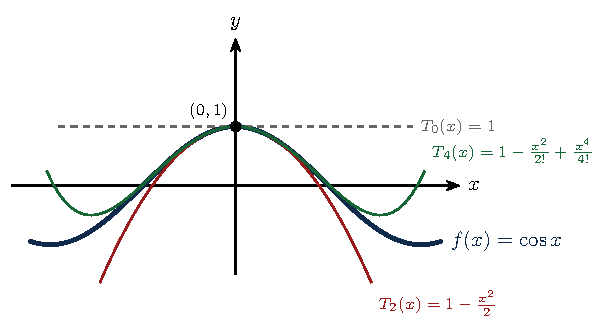
\includegraphics[width=0.88\textwidth]{07_taylor_polynomials.pdf}
  \caption{\textbf{Taylor Polynomial Approximations of $\cos x$ at $x_0 = 0$:} The zero-order polynomial $T_0(x) = 1$, second-order parabola $T_2(x) = 1 - \frac{x^2}{2}$, and fourth-order polynomial $T_4(x) = 1 - \frac{x^2}{2!} + \frac{x^4}{4!}$ progressively hug the true cosine curve over wider domains.}
  \label{fig:taylor_plots}
\end{figure}

\begin{theorembox}{Taylor-Young Formula (Local Expansion with Peano Remainder)}
If $f$ is $n$-times differentiable at $x_0$, then as $x \to x_0$:
\begin{equation}
f(x) = \sum_{k=0}^n \frac{f^{(k)}(x_0)}{k!} (x - x_0)^k + o\big((x - x_0)^n\big) \quad \text{as } x \to x_0,
\end{equation}
where $o\big((x - x_0)^n\big) = (x - x_0)^n \varepsilon(x)$ with $\lim_{x \to x_0} \varepsilon(x) = 0$ (Landau's small-$o$ notation).
\end{theorembox}

\section{Limited Developments (Développements Limités at $0$)}

\begin{definitionbox}{Limited Development of Order $n$ at $0$ ($\mathrm{DL}_n(0)$)}
A function $f$ admits a \textbf{limited development} of order $n \in \mathbb{N}$ in the neighborhood of $0$ if there exists a polynomial $P_n(x) = a_0 + a_1 x + a_2 x^2 + \dots + a_n x^n$ of degree $\le n$ such that:
\begin{equation}
f(x) = P_n(x) + x^n \varepsilon(x) \quad \text{with} \quad \lim_{x \to 0} \varepsilon(x) = 0.
\end{equation}
The polynomial $P_n(x)$ is \textbf{strictly unique}. If $f$ is $n$-times differentiable, $a_k = \frac{f^{(k)}(0)}{k!}$ (Maclaurin expansion).
\end{definitionbox}

\begin{propbox}{Reference Maclaurin Expansions at $x = 0$}
As $x \to 0$, the following standard limited developments hold:
\begin{align}
e^x &= 1 + x + \frac{x^2}{2!} + \frac{x^3}{3!} + \dots + \frac{x^n}{n!} + o(x^n) \\
\sin x &= x - \frac{x^3}{3!} + \frac{x^5}{5!} - \dots + (-1)^p \frac{x^{2p+1}}{(2p+1)!} + o(x^{2p+2}) \\
\cos x &= 1 - \frac{x^2}{2!} + \frac{x^4}{4!} - \dots + (-1)^p \frac{x^{2p}}{(2p)!} + o(x^{2p+1}) \\
\ln(1 + x) &= x - \frac{x^2}{2} + \frac{x^3}{3} - \frac{x^4}{4} + \dots + (-1)^{n-1} \frac{x^n}{n} + o(x^n) \\
(1 + x)^\alpha &= 1 + \alpha x + \frac{\alpha(\alpha-1)}{2!} x^2 + \dots + \frac{\alpha(\alpha-1)\cdots(\alpha-n+1)}{n!} x^n + o(x^n) \\
\frac{1}{1 - x} &= 1 + x + x^2 + x^3 + \dots + x^n + o(x^n) \\
\frac{1}{1 + x} &= 1 - x + x^2 - x^3 + \dots + (-1)^n x^n + o(x^n) \\
\arctan x &= x - \frac{x^3}{3} + \frac{x^5}{5} - \dots + (-1)^p \frac{x^{2p+1}}{2p+1} + o(x^{2p+2})
\end{align}
\end{propbox}

\section{The Riemann Integral and Fundamental Theorem of Calculus}

\begin{figure}[htbp]
  \centering
  \begin{minipage}{0.35\textwidth}
    \centering
    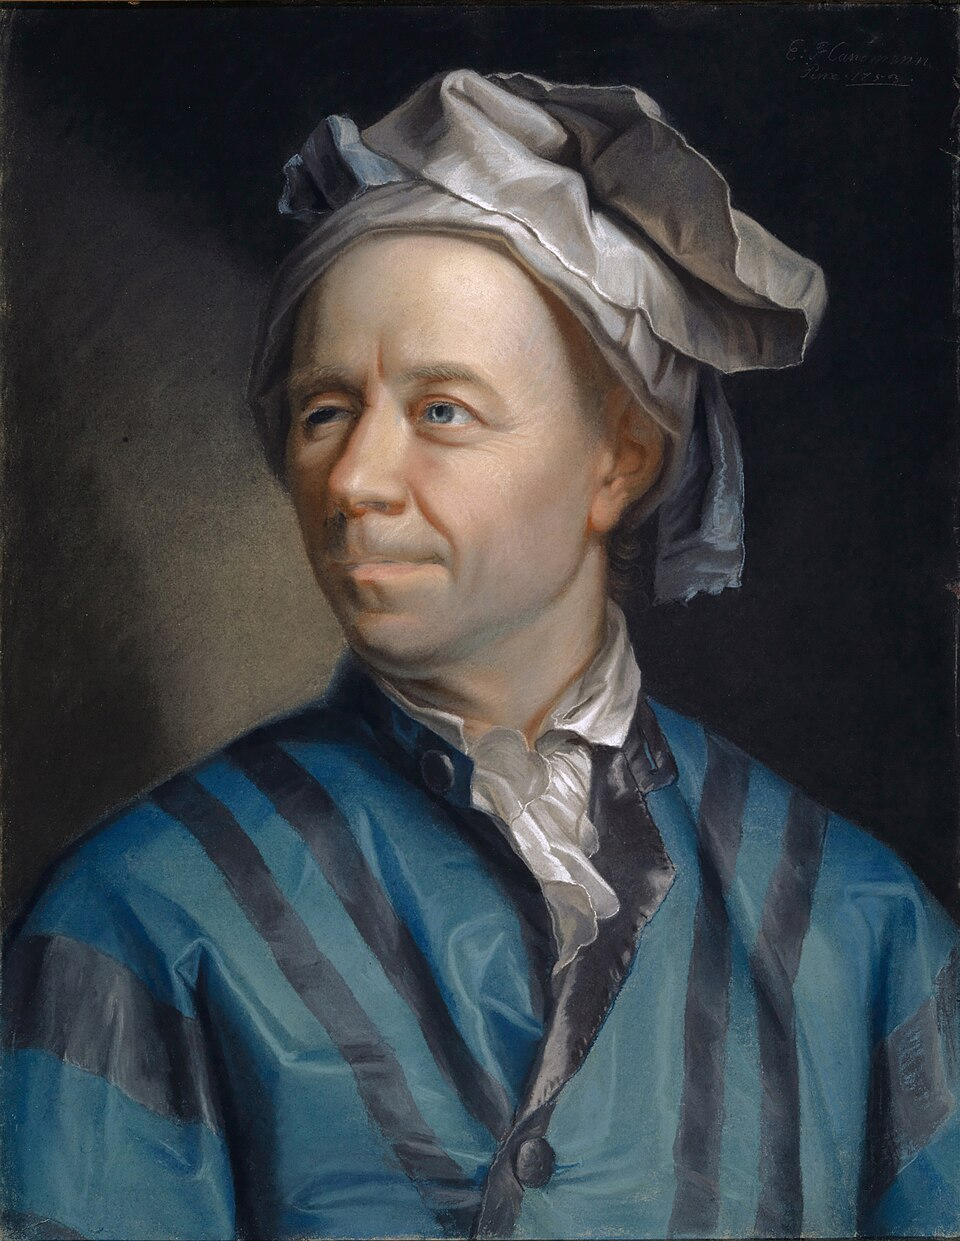
\includegraphics[width=0.82\textwidth]{euler.jpg}
    \caption*{(a) \textbf{Leonhard Euler (1707--1783)}}
  \end{minipage}
  \hspace{0.08\textwidth}
  \begin{minipage}{0.35\textwidth}
    \centering
    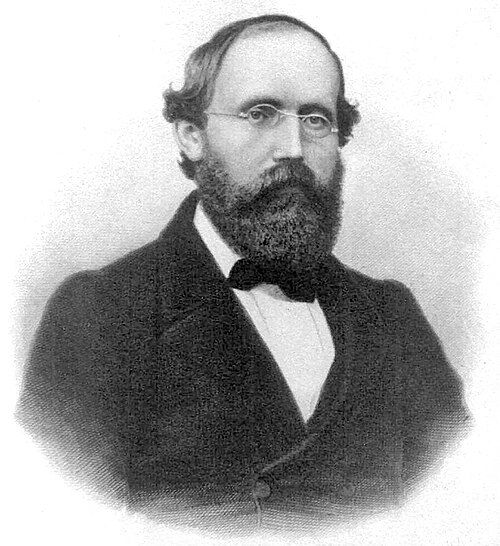
\includegraphics[width=0.82\textwidth]{riemann.jpg}
    \caption*{(b) \textbf{Bernhard Riemann (1826--1866)}}
  \end{minipage}
  \caption{\textbf{Pioneers of Integral Analysis:} Leonhard Euler (master of analytical transformations and infinite sums) and Bernhard Riemann (creator of the modern definition of the definite integral via partition step sums).}
  \label{fig:euler_riemann}
\end{figure}

\begin{definitionbox}{The Riemann Integral}
Let $f: [a, b] \longrightarrow \mathbb{R}$ be a bounded function.
A \textbf{subdivision} (partition) of $[a, b]$ is a finite ordered sequence $\sigma = \{a = x_0 < x_1 < x_2 < \dots < x_n = b\}$.
For any choice of evaluation tags $\xi_i \in [x_{i-1}, x_i]$, the \textbf{Riemann sum} is:
\begin{equation}
S(f, \sigma, \xi) = \sum_{i=1}^n f(\xi_i) \cdot (x_i - x_{i-1}) = \sum_{i=1}^n f(\xi_i) \Delta x_i.
\end{equation}
$f$ is \textbf{Riemann integrable} on $[a, b]$ if the Riemann sums converge to a unique real limit as the mesh size $\max_i \Delta x_i \to 0$:
\begin{equation}
\int_a^b f(x)\,\dd x = \lim_{\|\sigma\| \to 0} \sum_{i=1}^n f(\xi_i) \Delta x_i.
\end{equation}
\textbf{Integrability Criterion:} Every continuous function on $[a, b]$ ($f \in \mathcal{C}^0([a, b])$) and every piecewise continuous monotonic function is Riemann integrable.
\end{definitionbox}

\begin{figure}[htbp]
  \centering
  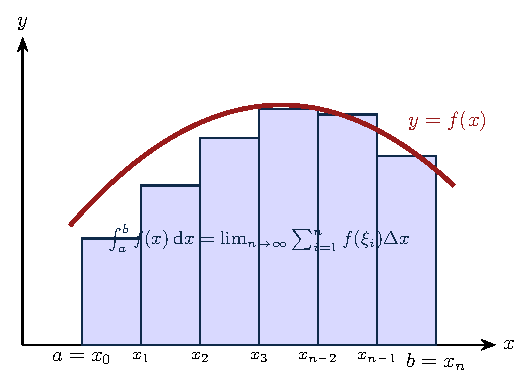
\includegraphics[width=0.88\textwidth]{08_riemann_integral.pdf}
  \caption{\textbf{Riemann Integral as the Limit of Rectangular Approximations:} Subdividing $[a, b]$ into $n$ subintervals and summing the areas of rectangular slices converges to the exact geometric area under $y = f(x)$.}
  \label{fig:riemann_rectangles}
\end{figure}

\begin{theorembox}{The Fundamental Theorem of Calculus (FTC)}
\begin{enumerate}[leftmargin=1.4em,itemsep=3pt]
  \item \textbf{First Part (Existence of Antiderivatives):}
  Let $f: [a, b] \longrightarrow \mathbb{R}$ be continuous. The function $F: [a, b] \longrightarrow \mathbb{R}$ defined by:
  \[
  F(x) = \int_a^x f(t)\,\dd t
  \]
  is continuous on $[a, b]$, differentiable on $(a, b)$, and its derivative is identically $f$:
  \[
  F'(x) = \frac{\dd}{\dd x} \left( \int_a^x f(t)\,\dd t \right) = f(x) \quad \text{for all } x \in [a, b].
  \]
  \item \textbf{Second Part (Newton-Leibniz Formula):}
  If $G$ is any antiderivative of $f$ on $[a, b]$ (so $G'(x) = f(x)$):
  \begin{equation}
  \int_a^b f(t)\,\dd t = G(b) - G(a) = \big[ G(t) \big]_a^b.
  \end{equation}
\end{enumerate}
\end{theorembox}

\begin{propbox}{Essential Integration Techniques}
\begin{enumerate}[leftmargin=1.4em,itemsep=3pt]
  \item \textbf{Integration by Parts (IPP):}
  Let $u, v \in \mathcal{C}^1([a, b])$:
  \begin{equation}
  \int_a^b u(t) v'(t)\,\dd t = \big[ u(t) v(t) \big]_a^b - \int_a^b u'(t) v(t)\,\dd t.
  \end{equation}
  \item \textbf{Integration by Substitution (Change of Variable):}
  Let $\phi: [\alpha, \beta] \longrightarrow [a, b]$ be a function of class $\mathcal{C}^1$ with $\phi(\alpha) = a$ and $\phi(\beta) = b$, and let $f \in \mathcal{C}^0([a, b])$:
  \begin{equation}
  \int_a^b f(x)\,\dd x = \int_\alpha^\beta f(\phi(t)) \cdot \phi'(t)\,\dd t.
  \end{equation}
\end{enumerate}
\end{propbox}

\section{Worked Examples with Step-by-Step Proofs}

\begin{workedexample}{High-Order Derivative Using Leibniz's Product Rule}
Compute the $n$-th derivative of the function:
\[
f(x) = x^2 e^{3x}.
\]

\paragraph{Solution and Proof.}
Write $f(x) = u(x) \cdot v(x)$ where:
\[
u(x) = x^2, \qquad v(x) = e^{3x}.
\]
Compute the successive derivatives of $u(x)$:
\[
u^{(0)}(x) = x^2, \quad u^{(1)}(x) = 2x, \quad u^{(2)}(x) = 2, \quad \text{and} \quad u^{(k)}(x) = 0 \quad \text{for all } k \ge 3.
\]
Compute the successive derivatives of $v(x)$:
\[
v^{(k)}(x) = 3^k e^{3x} \quad \text{for all } k \ge 0.
\]
Applying **Leibniz's Formula**:
\[
f^{(n)}(x) = \sum_{k=0}^n \binom{n}{k} u^{(k)}(x) v^{(n-k)}(x).
\]
Since $u^{(k)}(x) = 0$ for all $k \ge 3$, only the first three terms ($k = 0, 1, 2$) survive:
\begin{align*}
f^{(n)}(x) &= \binom{n}{0} u(x) v^{(n)}(x) + \binom{n}{1} u'(x) v^{(n-1)}(x) + \binom{n}{2} u''(x) v^{(n-2)}(x) \\
           &= 1 \cdot (x^2) \cdot \left( 3^n e^{3x} \right) + n \cdot (2x) \cdot \left( 3^{n-1} e^{3x} \right) + \frac{n(n-1)}{2} \cdot (2) \cdot \left( 3^{n-2} e^{3x} \right).
\end{align*}
Factor out the common exponential and power term $3^{n-2} e^{3x}$:
\begin{align*}
f^{(n)}(x) &= 3^{n-2} e^{3x} \left[ 3^2 x^2 + 2n \cdot 3 x + n(n-1) \right] \\
           &= \mathbf{3^{n-2} e^{3x} \left[ 9x^2 + 6nx + n(n-1) \right]}. \quad \blacksquare
\end{align*}
\end{workedexample}

\begin{workedexample}{Indeterminate Limit via Limited Development}
Compute using limited developments the limit:
\[
L = \lim_{x \to 0} \frac{\sin x - x \cos x}{x^3}.
\]

\paragraph{Solution and Proof.}
As $x \to 0$, the numerator approaches $\sin 0 - 0 = 0$ and the denominator $x^3 \to 0$, producing an indeterminate form of type $\left[ \frac{0}{0} \right]$.
Since the denominator is of degree $3$, we expand the numerator to order $3$ ($\mathrm{DL}_3(0)$).

Recall the reference Maclaurin expansions to order $3$:
\begin{align*}
\sin x &= x - \frac{x^3}{6} + o(x^3), \\
\cos x &= 1 - \frac{x^2}{2} + o(x^2).
\end{align*}
Multiply $\cos x$ by $x$:
\[
x \cos x = x \left( 1 - \frac{x^2}{2} + o(x^2) \right) = x - \frac{x^3}{2} + o(x^3).
\]
Subtract the two expressions:
\begin{align*}
\sin x - x \cos x &= \left( x - \frac{x^3}{6} + o(x^3) \right) - \left( x - \frac{x^3}{2} + o(x^3) \right) \\
                  &= (x - x) + \left( -\frac{1}{6} + \frac{1}{2} \right) x^3 + o(x^3) \\
                  &= \left( -\frac{1}{6} + \frac{3}{6} \right) x^3 + o(x^3) = \frac{2}{6} x^3 + o(x^3) = \frac{1}{3} x^3 + o(x^3).
\end{align*}
Now divide by the denominator $x^3$:
\[
\frac{\sin x - x \cos x}{x^3} = \frac{\frac{1}{3} x^3 + o(x^3)}{x^3} = \frac{1}{3} + \frac{o(x^3)}{x^3} = \frac{1}{3} + \varepsilon(x),
\]
where $\lim_{x \to 0} \varepsilon(x) = 0$.
Taking the limit as $x \to 0$:
\[
\mathbf{L = \lim_{x \to 0} \frac{\sin x - x \cos x}{x^3} = \frac{1}{3}}. \quad \blacksquare
\]
\end{workedexample}

\begin{workedexample}{Integration by Parts: Wallis Integrals}
Consider the sequence of \textbf{Wallis Integrals} defined for $n \in \mathbb{N}$ by:
\[
W_n = \int_0^{\pi/2} \sin^n(x)\,\dd x.
\]
\begin{enumerate}[leftmargin=1.4em,itemsep=2pt]
  \item Compute $W_0$ and $W_1$.
  \item Using integration by parts, establish the recurrence relation:
  \[
  W_n = \frac{n - 1}{n} W_{n-2} \quad \text{for all } n \ge 2.
  \]
\end{enumerate}

\paragraph{Solution and Proof.}
\textbf{1. Direct Evaluation of $W_0$ and $W_1$:}
\[
W_0 = \int_0^{\pi/2} 1\,\dd x = [x]_0^{\pi/2} = \mathbf{\frac{\pi}{2}}.
\]
\[
W_1 = \int_0^{\pi/2} \sin x\,\dd x = [-\cos x]_0^{\pi/2} = -\cos(\pi/2) - (-\cos 0) = 0 - (-1) = \mathbf{1}.
\]

\textbf{2. Integration by Parts for $n \ge 2$:}
Split the integrand: $\sin^n x = \sin^{n-1} x \cdot \sin x$.
Set:
\begin{align*}
u(x) &= \sin^{n-1} x \implies u'(x) = (n-1) \sin^{n-2} x \cos x, \\
v'(x) &= \sin x \implies v(x) = -\cos x.
\end{align*}
Applying the integration by parts formula:
\[
W_n = \big[ -\sin^{n-1}(x) \cos(x) \big]_0^{\pi/2} - \int_0^{\pi/2} (n-1) \sin^{n-2}(x) \cos(x) \cdot (-\cos x)\,\dd x.
\]
Evaluate the boundary bracket:
\begin{itemize}[itemsep=1pt]
  \item At $x = \pi/2$: $\cos(\pi/2) = 0$.
  \item At $x = 0$: for $n \ge 2$, $n - 1 \ge 1$, so $\sin^{n-1}(0) = 0$.
\end{itemize}
Thus the boundary term vanishes identically: $\big[ -\sin^{n-1}(x) \cos(x) \big]_0^{\pi/2} = 0$.
The integral term becomes:
\[
W_n = (n - 1) \int_0^{\pi/2} \sin^{n-2}(x) \cos^2(x)\,\dd x.
\]
Substitute the trigonometric identity $\cos^2 x = 1 - \sin^2 x$:
\begin{align*}
W_n &= (n - 1) \int_0^{\pi/2} \sin^{n-2}(x) (1 - \sin^2 x)\,\dd x \\
    &= (n - 1) \int_0^{\pi/2} \sin^{n-2}(x)\,\dd x - (n - 1) \int_0^{\pi/2} \sin^n(x)\,\dd x \\
    &= (n - 1) W_{n-2} - (n - 1) W_n.
\end{align*}
Rearranging terms in $W_n$:
\[
W_n + (n - 1) W_n = (n - 1) W_{n-2} \implies n W_n = (n - 1) W_{n-2}.
\]
Dividing across by $n > 0$:
\[
\mathbf{W_n = \frac{n - 1}{n} W_{n-2}}. \quad \blacksquare
\]
\end{workedexample}

\begin{workedexample}{Integration by Rational Substitution}
Compute the definite integral:
\[
I = \int_0^1 \frac{\dd x}{1 + \sqrt{x}}.
\]

\paragraph{Solution and Proof.}
The presence of the square root radical $\sqrt{x}$ suggests the change of variable:
\[
u = \sqrt{x} \iff x = u^2.
\]
Differentiating both sides:
\[
\dd x = 2u\,\dd u.
\]
Determine the new integration bounds:
\begin{itemize}[itemsep=1pt]
  \item When $x = 0$: $u = \sqrt{0} = 0$.
  \item When $x = 1$: $u = \sqrt{1} = 1$.
\end{itemize}
Substitute into the integral:
\[
I = \int_0^1 \frac{2u\,\dd u}{1 + u} = 2 \int_0^1 \frac{u}{u + 1}\,\dd u.
\]
Perform algebraic decomposition of the rational integrand by adding and subtracting $1$:
\[
\frac{u}{u + 1} = \frac{(u + 1) - 1}{u + 1} = 1 - \frac{1}{u + 1}.
\]
Now integrate term by term:
\begin{align*}
I &= 2 \int_0^1 \left( 1 - \frac{1}{u + 1} \right)\,\dd u = 2 \Big[ u - \ln(u + 1) \Big]_0^1 \\
  &= 2 \Big[ (1 - \ln 2) - (0 - \ln 1) \Big] \\
  &= 2(1 - \ln 2) = \mathbf{2 - 2 \ln 2} \approx \mathbf{0.6137}. \quad \blacksquare
\end{align*}
\end{workedexample}

\chapter{Mathematical Reference Tables and Formula Manual}
\label{app:math_tables}

\section{Master Table of Standard Derivatives}

\renewcommand{\arraystretch}{1.3}
\begin{longtable}{@{}lll@{}}
\toprule
\textbf{Function} $f(x)$ & \textbf{Derivative} $f'(x)$ & \textbf{Domain of Differentiability} \\
\midrule
\endhead
Constant: $c$ & $0$ & $\mathbb{R}$ \\
Power: $x^n$ ($n \in \mathbb{Z}$) & $n x^{n-1}$ & $\mathbb{R}$ (or $\mathbb{R}^*$ if $n < 0$) \\
Power: $x^\alpha$ ($\alpha \in \mathbb{R}$) & $\alpha x^{\alpha-1}$ & $(0, +\infty)$ \\
Square root: $\sqrt{x}$ & $\dfrac{1}{2\sqrt{x}}$ & $(0, +\infty)$ \\
Natural exponential: $e^x$ & $e^x$ & $\mathbb{R}$ \\
General exponential: $a^x$ ($a > 0$) & $a^x \ln(a)$ & $\mathbb{R}$ \\
Natural logarithm: $\ln|x|$ & $\dfrac{1}{x}$ & $\mathbb{R}^*$ \\
Sine: $\sin(x)$ & $\cos(x)$ & $\mathbb{R}$ \\
Cosine: $\cos(x)$ & $-\sin(x)$ & $\mathbb{R}$ \\
Tangent: $\tan(x)$ & $1 + \tan^2(x) = \dfrac{1}{\cos^2(x)}$ & $x \neq \dfrac{\pi}{2} + k\pi$ \\
Arcsine: $\arcsin(x)$ & $\dfrac{1}{\sqrt{1 - x^2}}$ & $(-1, 1)$ \\
Arccosine: $\arccos(x)$ & $-\dfrac{1}{\sqrt{1 - x^2}}$ & $(-1, 1)$ \\
Arctangent: $\arctan(x)$ & $\dfrac{1}{1 + x^2}$ & $\mathbb{R}$ \\
Hyperbolic sine: $\sinh(x)$ & $\cosh(x)$ & $\mathbb{R}$ \\
Hyperbolic cosine: $\cosh(x)$ & $\sinh(x)$ & $\mathbb{R}$ \\
Hyperbolic tangent: $\tanh(x)$ & $1 - \tanh^2(x) = \dfrac{1}{\cosh^2(x)}$ & $\mathbb{R}$ \\
\bottomrule
\end{longtable}

\section{Master Table of Indefinite Integrals (Antiderivatives)}

\renewcommand{\arraystretch}{1.35}
\begin{longtable}{@{}lll@{}}
\toprule
\textbf{Integrand} $f(x)$ & \textbf{General Antiderivative} $\int f(x)\,\dd x$ & \textbf{Validity Interval} \\
\midrule
\endhead
$x^\alpha$ ($\alpha \neq -1$) & $\dfrac{x^{\alpha+1}}{\alpha + 1} + C$ & $(0, +\infty)$ \\
$\dfrac{1}{x}$ & $\ln|x| + C$ & $(-\infty, 0)$ or $(0, +\infty)$ \\
$e^{\lambda x}$ ($\lambda \neq 0$) & $\dfrac{1}{\lambda} e^{\lambda x} + C$ & $\mathbb{R}$ \\
$\sin(x)$ & $-\cos(x) + C$ & $\mathbb{R}$ \\
$\cos(x)$ & $\sin(x) + C$ & $\mathbb{R}$ \\
$\dfrac{1}{\cos^2(x)} = 1 + \tan^2(x)$ & $\tan(x) + C$ & $(-\pi/2, \pi/2) + k\pi$ \\
$\dfrac{1}{1 + x^2}$ & $\arctan(x) + C$ & $\mathbb{R}$ \\
$\dfrac{1}{a^2 + x^2}$ ($a > 0$) & $\dfrac{1}{a} \arctan\left(\dfrac{x}{a}\right) + C$ & $\mathbb{R}$ \\
$\dfrac{1}{\sqrt{1 - x^2}}$ & $\arcsin(x) + C$ & $(-1, 1)$ \\
$\dfrac{1}{\sqrt{a^2 - x^2}}$ ($a > 0$) & $\arcsin\left(\dfrac{x}{a}\right) + C$ & $(-a, a)$ \\
$\dfrac{1}{\sqrt{x^2 + 1}}$ & $\mathrm{argsinh}(x) + C = \ln\left(x + \sqrt{x^2 + 1}\right) + C$ & $\mathbb{R}$ \\
$\dfrac{1}{\sqrt{x^2 - 1}}$ & $\mathrm{argcosh}(x) + C = \ln\left(x + \sqrt{x^2 - 1}\right) + C$ & $(1, +\infty)$ \\
$\dfrac{u'(x)}{u(x)}$ & $\ln|u(x)| + C$ & where $u(x) \neq 0$ \\
$u'(x) [u(x)]^\alpha$ ($\alpha \neq -1$) & $\dfrac{[u(x)]^{\alpha+1}}{\alpha + 1} + C$ & where $u(x)$ valid \\
$u'(x) e^{u(x)}$ & $e^{u(x)} + C$ & $\mathbb{R}$ \\
\bottomrule
\end{longtable}

\section{Master Table of Asymptotic Equivalents as $x \to 0$}

\begin{center}
\renewcommand{\arraystretch}{1.3}
\begin{tabular}{@{}ll@{}}
\toprule
\textbf{Expression} & \textbf{Equivalent as } $x \to 0$ \\
\midrule
$\sin(x)$ & $x$ \\
$\tan(x)$ & $x$ \\
$\arcsin(x)$ & $x$ \\
$\arctan(x)$ & $x$ \\
$\sinh(x)$ & $x$ \\
$\tanh(x)$ & $x$ \\
$1 - \cos(x)$ & $\dfrac{x^2}{2}$ \\
$\cosh(x) - 1$ & $\dfrac{x^2}{2}$ \\
$e^x - 1$ & $x$ \\
$\ln(1 + x)$ & $x$ \\
$(1 + x)^\alpha - 1$ & $\alpha x$ \\
$\sqrt{1 + x} - 1$ & $\dfrac{x}{2}$ \\
\bottomrule
\end{tabular}
\end{center}


\end{document}
